% Chapter2

\chapter{State of the Art} \label{chapter:stateoftheart}

	% ##################################################################
	% Definition Prozessen, für die späterer Verwendung der Worte 
	% ##################################################################

	\section{Konzeptionelle Planung einer Anlage}
	Es ist gängige Praxis in der Anlagen- und Verfahrenstechnik, vor Realisierung der Anlage eine schematische Darstellung zu modellieren. Das Rohr- und Instrumentenfließschema ist ein probates Mittel für die Erstellung eines vollständiges Abbildes. Die verwendeten Bauteile sind jedenfalls namentlich beschriftet, können aber auch zusätzliche Informationen, die zum Verständnis der Verwendung beitragen, beinhalten. Das beschriebene Schema ist im Standard \todo{Welcher Standard?} wie folgt niedergeschrieben \todo[color=green]{Lepu: Wo ist der Standard niedergeschrieben?}\\
	
	Zur Anwendung kommt der beschriebene Arbeitsschritt beispielsweise bei einem Reaktor, welcher die hinreichende Bedingung \glqq Name \grqq \space und darüber hinaus fakultative Invarianten wie Anzahl und Lokalisation der Ein- und Ausgänge hat. Weiteres könnten auch Angaben zur Implementierung von Sensoren oder Aktoren vermerkt sein. Rohre werden im Rohr- und Instrumentenfließschema als Verbindungslinien zwischen Bauteilen dargestellt. Detailinformationen wie Nenndruck, Rohrklasse oder Spezifikationsnummer können ergänzend vermerkt werden. Somit sind in einem Rohr- und Instrumentenfließschema Apparate (Tanks, Speicherbehälter, Reaktoren, o. Ä.), Maschinen (Pumpen, Verdichter, o. Ä.) und Leitungen darstellbar.\\
	
	Die folgende Abbildung~\ref{fig:RI_SotA} zeigt den Aufbau einer simplen Anlage mit Hilfe des Rohr- und Instrumentenfließschemas.\\

	\begin{figure}[h!]
  		\centering
		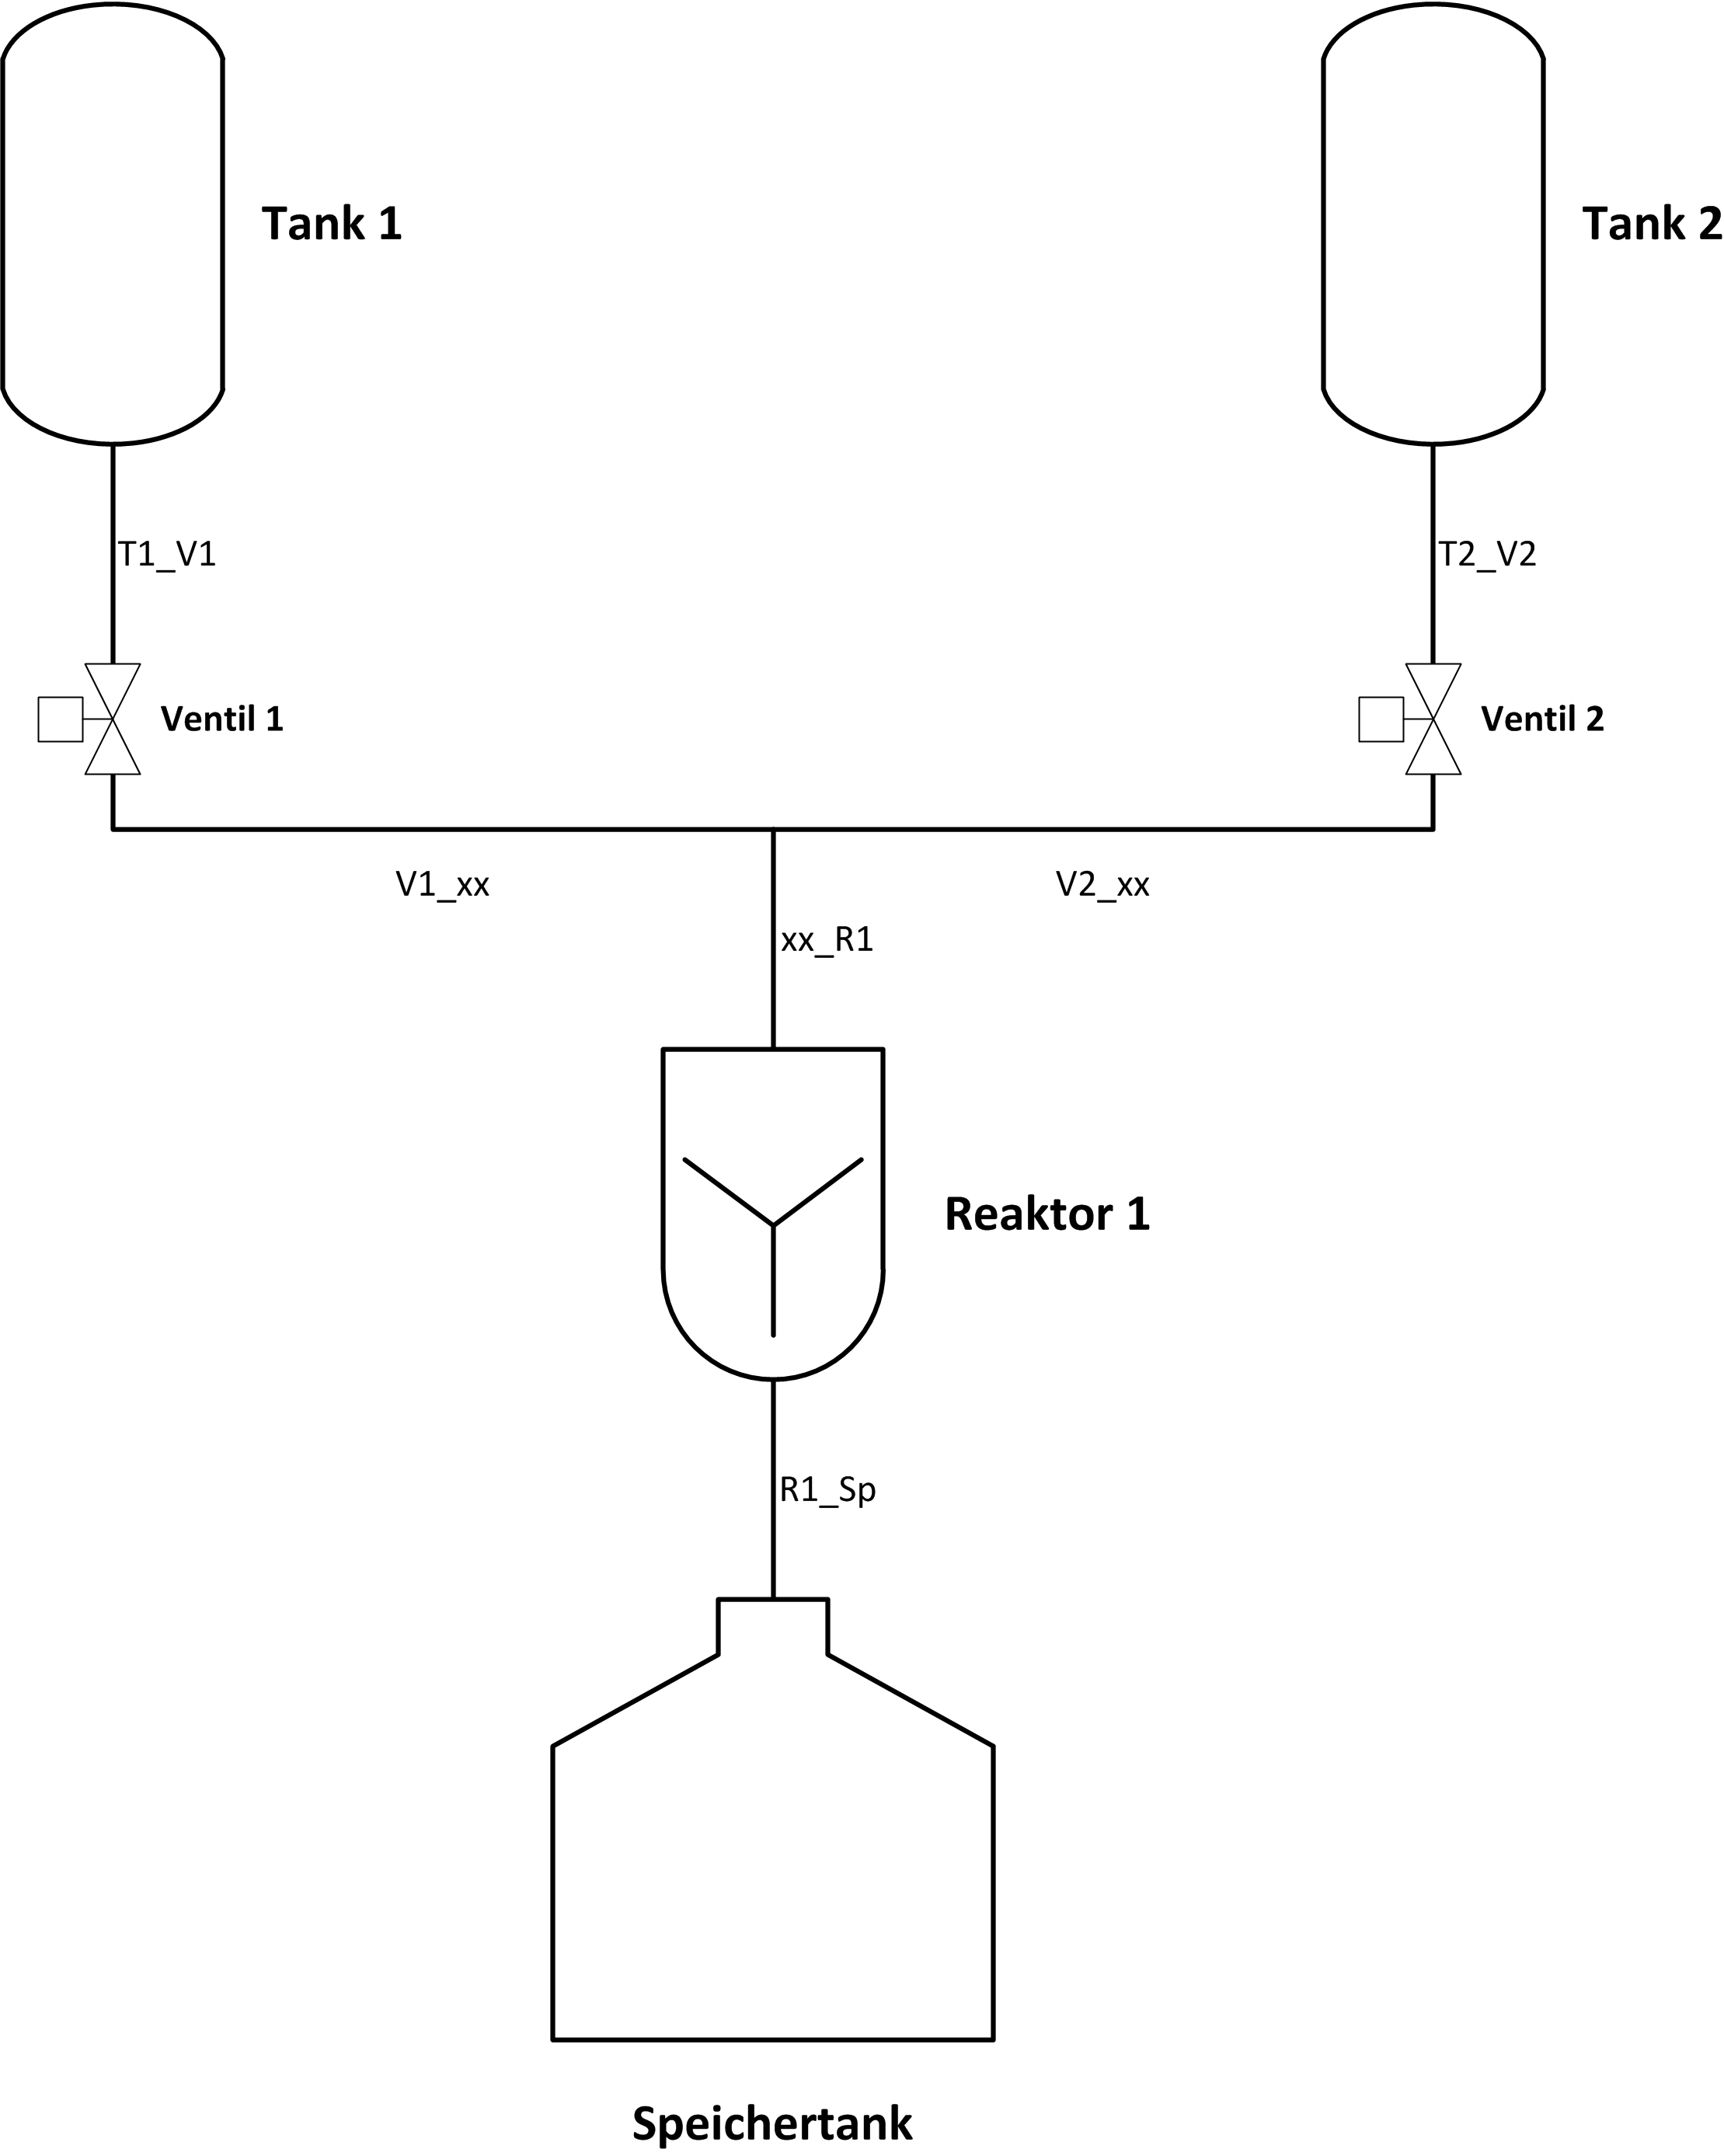
\includegraphics[height=0.7\textwidth]{graphics/stateoftheart/RI_SotA.jpg}
		\caption{Rohr- und Instrumentenfließschema}
		\label{fig:RI_SotA}
	\end{figure}

	\newpage
	\section{Definition eines Prozesses}
	Ein Prozess ist dadurch definiert, welche Arbeitsschritte bewerkstelligt werden müssen, um als Ergebnis das gewünschte Produkt zu erlangen. Die Anforderungen beziehungsweise das Zielprodukt formt somit den Arbeitsprozess.
	
	\begin{figure}[h!]
  		\centering
		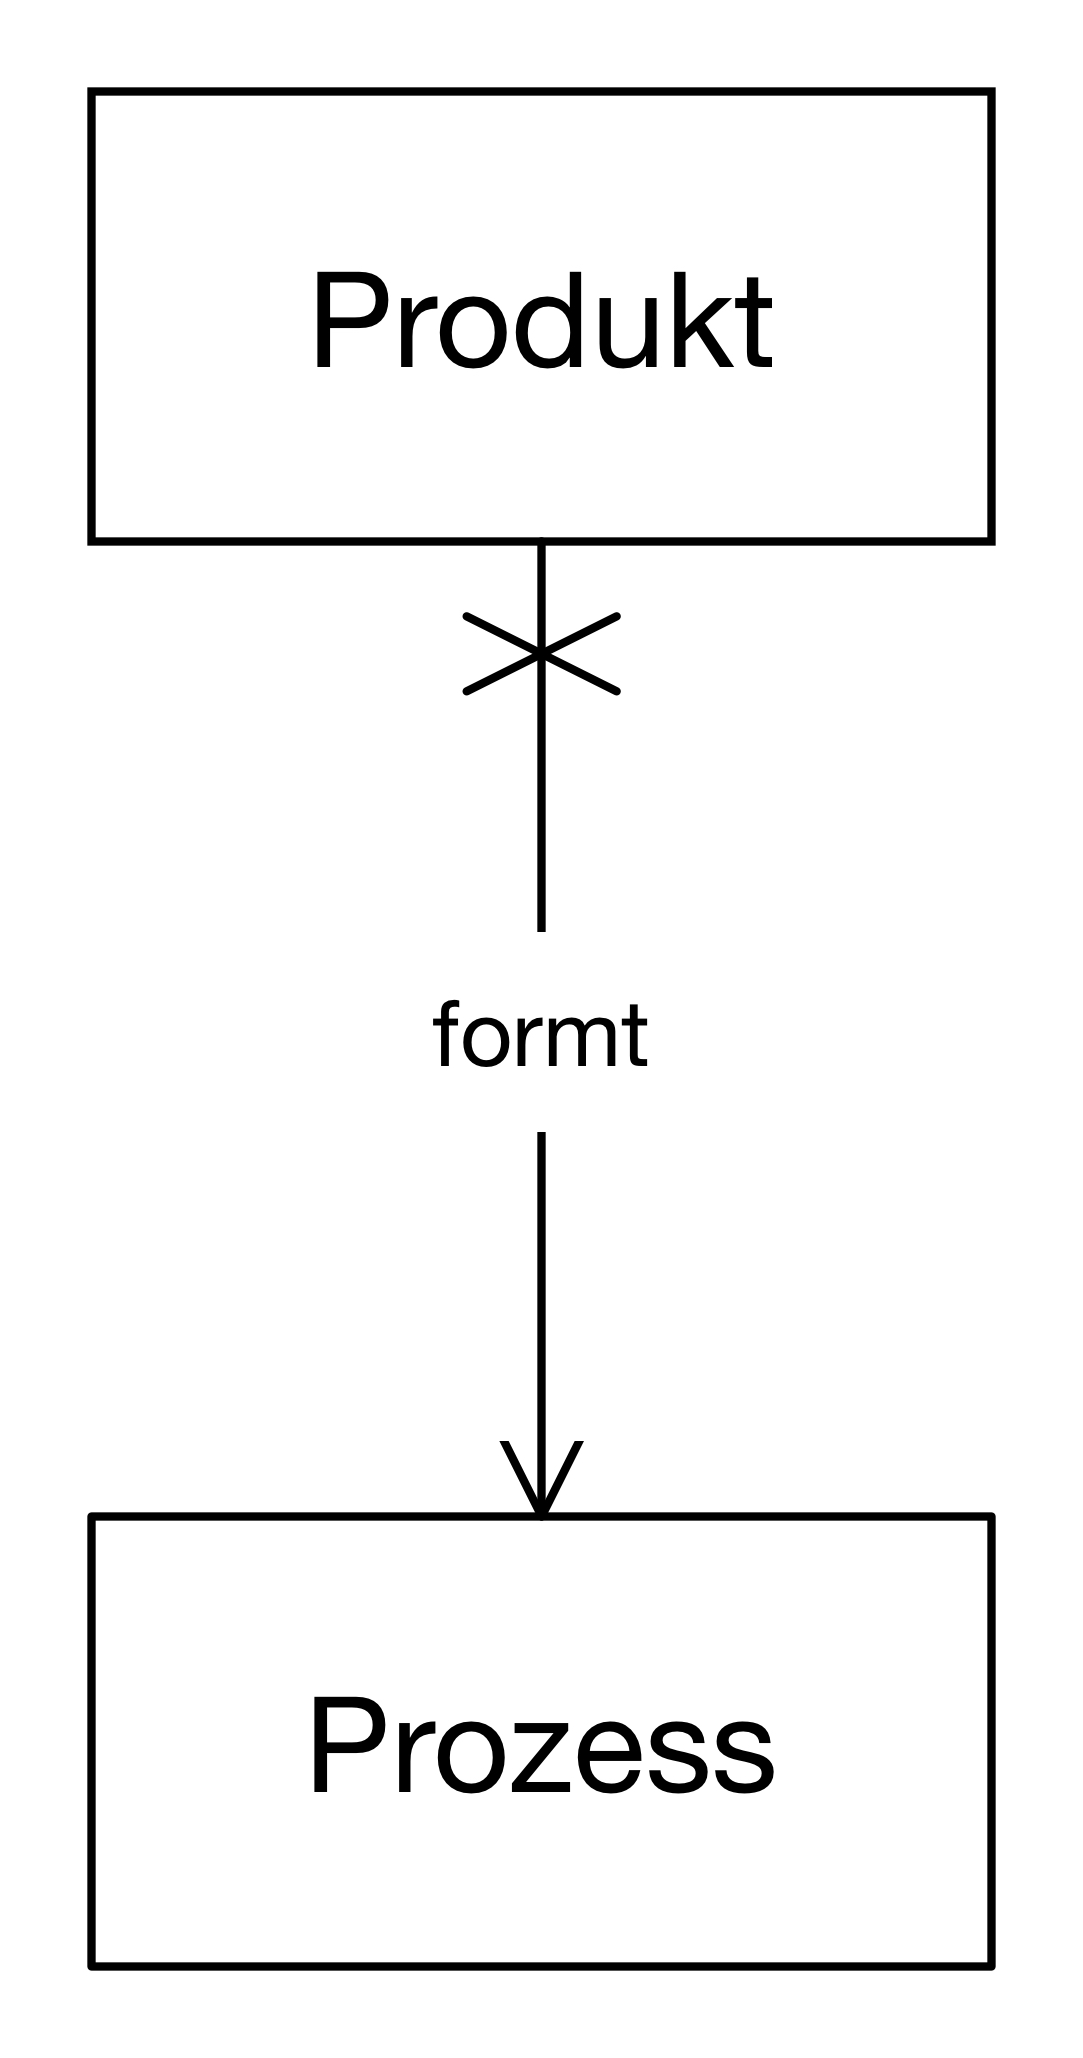
\includegraphics[height=0.5\textwidth]{graphics/stateoftheart/Prozess.jpg}
		\caption{Definition eines Prozess}
	\end{figure}
	
	Laut der Norm DIN IEC 60050-351 ist ein Prozess wie folgt definiert \cite{mpolke_proc}:\\
	
	\todo[inline]{Lepu fragen ob diese Zitierungsart ok ist}
	
	\textit{Ein Prozess repräsentiert einen Ablauf von sequentiell ausgeführten Aktivitäten innerhalb eines Systems zum Umwandeln, Lagern und Transportieren von Material, Energie oder Informationen.}\\

	Dabei ist wiederum tiefer ins Detail zu gehen, da es für technische Prozesse eine eigens entworfene, genauer spezifizierende Definition gibt.\\
	
	\textit{Ein technischer Prozess ist ein Prozess, dessen physikalische Werte gemessen, sowie mit technischen Mitteln beeinflusst werden.}\\
	
	Zu unterscheiden ist zwischen folgenden Prozessen:
	
	\begin{itemize}
		\item Diskreter Prozess
		\item Kontinuierlicher Prozess
		\item Chargenprozess
	\end{itemize}
	
	\subsection{Diskreter Prozess}
	Der diskrete Prozess wird häufig auch als \glqq Fertigungsprozess\grqq\space definiert, wobei es sich dabei im Grunde genommen um dasselbe handelt. Zu den Eigenschaften solch eines Prozesses gehört ein klar definierter Start- und Endzeitpunkt. Der grundlegende Unterschied zu den noch folgenden ist jener, dass ausschließlich bei diskreten Prozessen die Formveränderung praktiziert wird, was wiederum bedeutet, dass es zu keiner stofflichen Strukturveränderung während des gesamten Ablaufs kommt. Zur Anwendung kommt diese Art in der Fertigung von mechanischen Produkten, wie etwa konkret in der Automobilindustrie.
	
	\subsection{Kontinuierliche Prozess}
	Konträr zum diskreten Prozess steht der häufig bei der Stromerzeugung zum Einsatz kommende kontinuierliche Prozess. Hierbei gibt es keinerlei festgeschriebenen Anfangs- und Endzeitpunkt, was zur Folge hat, dass an jedem Ort immer die selben Zustände auftreten, wobei der Betrachtungszeitpunkt irrelevant ist. Bei diesen oft auch als stationär bezeichneten Prozessen wird etwa zu Beginn einer Produktionskette stets der selbe Zustand des Produkts auftreten. Dabei beschränkt sich die Verarbeitung auf formlose Stoffe, die Sand, Flüssigkeiten oder Ähnliches sein können. Es kommt lediglich zu einer stofflichen Veränderung, wie einer chemischen Reaktion oder dem Aufheizen beziehungsweise Mischen mit einer anderen Substanz.
	
	\subsection{Chargenprozess}
	Bei der dritten und letzten Beschreibung handelt es sich um eine Art von Prozess, die teilweise Parallelen zu den diskreten und kontinuierlichen Prozesse aufweist. So wird abermals mit formlosen Materialien gearbeitet, welche ausschließlich stofflich verändert werden. Der ausschlaggebende Unterschied zu kontinuierlichen Prozessen ist jedoch, dass es klare Anfangs- und Endzeitpunkte während des Prozesses gibt. So hat etwa das Füllen eines Tanks ein eindeutiges Endergebnis, über das nicht folgenlos hinausgegangen werden kann.\\

	Ableitbar aus den obigen Definitionen müssen Anlagen auf Basis spezifischer Prozesse geplant und erbaut werden. Die Anlage hat hingegen keinen Selbstzweck, sondern dient einzig und alleine nur dafür, einen oder mehrere Prozesse zu realisieren.\\

	% ##################################################################
	% Warum welche Hardware (Kriterien für unsere Nutzung, Umsetzbarkeit
	% ##################################################################
	\section{Hardwareaufbau einer SPS}
	
	Um die im späteren Verlauf aufbauende Hardware genauer beschreiben zu können, muss zu Beginn ein wenig thematisch ausgeholt werden. So hat der Begriff der Steuerung einen undenkbar hohen Stellenwert, welcher ebenso geklärt gehört.\\

	Unter einer Prozess- Steuerung versteht man nach der Norm DIN 19226 einen Vorgang, bei dem durch Rückführen gemessener Prozesszustände, verglichen mit von der speicherprogrammierbaren Steuerung formulierten Parametern, Sollwerte zur Beeinflussung des gesamten Prozesses erzeugt werden. Im Gegensatz zu einer Regelung muss der von einem Sensor ausgelesene Ist-Wert jedoch nicht zwanghaft rückgeführt werden. Dies ist in Abbildung~\ref{fig:Aufbau_Steuerkreis_Selfmade} ersichtlich.\cite{mseitz_sps}\\
	
	Der Steuerkreis besteht aus Sensoren, einem Steuerungsrechner, welcher meistens mittels einer SPS realisiert wird, sowie Aktoren. Die Steuerungseinheit selbst ist ein Rechner mit dem Hauptaufgabenbereich, die programmierten, im Speicher abgelegten Anweisungen zyklisch auszuführen und über einfach anzusprechende Schnittstellen Daten einzulesen oder auszugeben. \cite{mseitz_sps} \\
	
	Der Begriff SPS wird in der Norm DIN EN 61131-1 (IEC 61131-1) wie folgt definiert:\\
	
	\glqq \textit{Ein digital arbeitendes elektronisches System für den Einsatz in industriellen Umgebungen mit einem programmierbaren Speicher zur internen Speicherung der anwenderorientierten Steuerungsanweisungen zur Implementierung spezifischer Funktionen wie z.B. Verknüpfungssteuerung, Ablaufsteuerung, Zeit-, Zähl- und arithmetische Funktionen, um durch digitale oder analoge Eingangs- und Ausgangssignale verschiedene Arten von Maschinen und Prozesse zu steuern. Die Speicherprogrammierbare Steuerung und die zugehörige Peripheriegerät (das SPS- System) sind so konzipiert, dass sie sich leicht in ein industrielles Steuerungssystem integrieren und in allen ihren beabsichtigten Funktionen einsetzen lassen.}\grqq \space \cite{sps_programmierung}\\
 
 	\begin{figure}[h!]
  		\centering
      	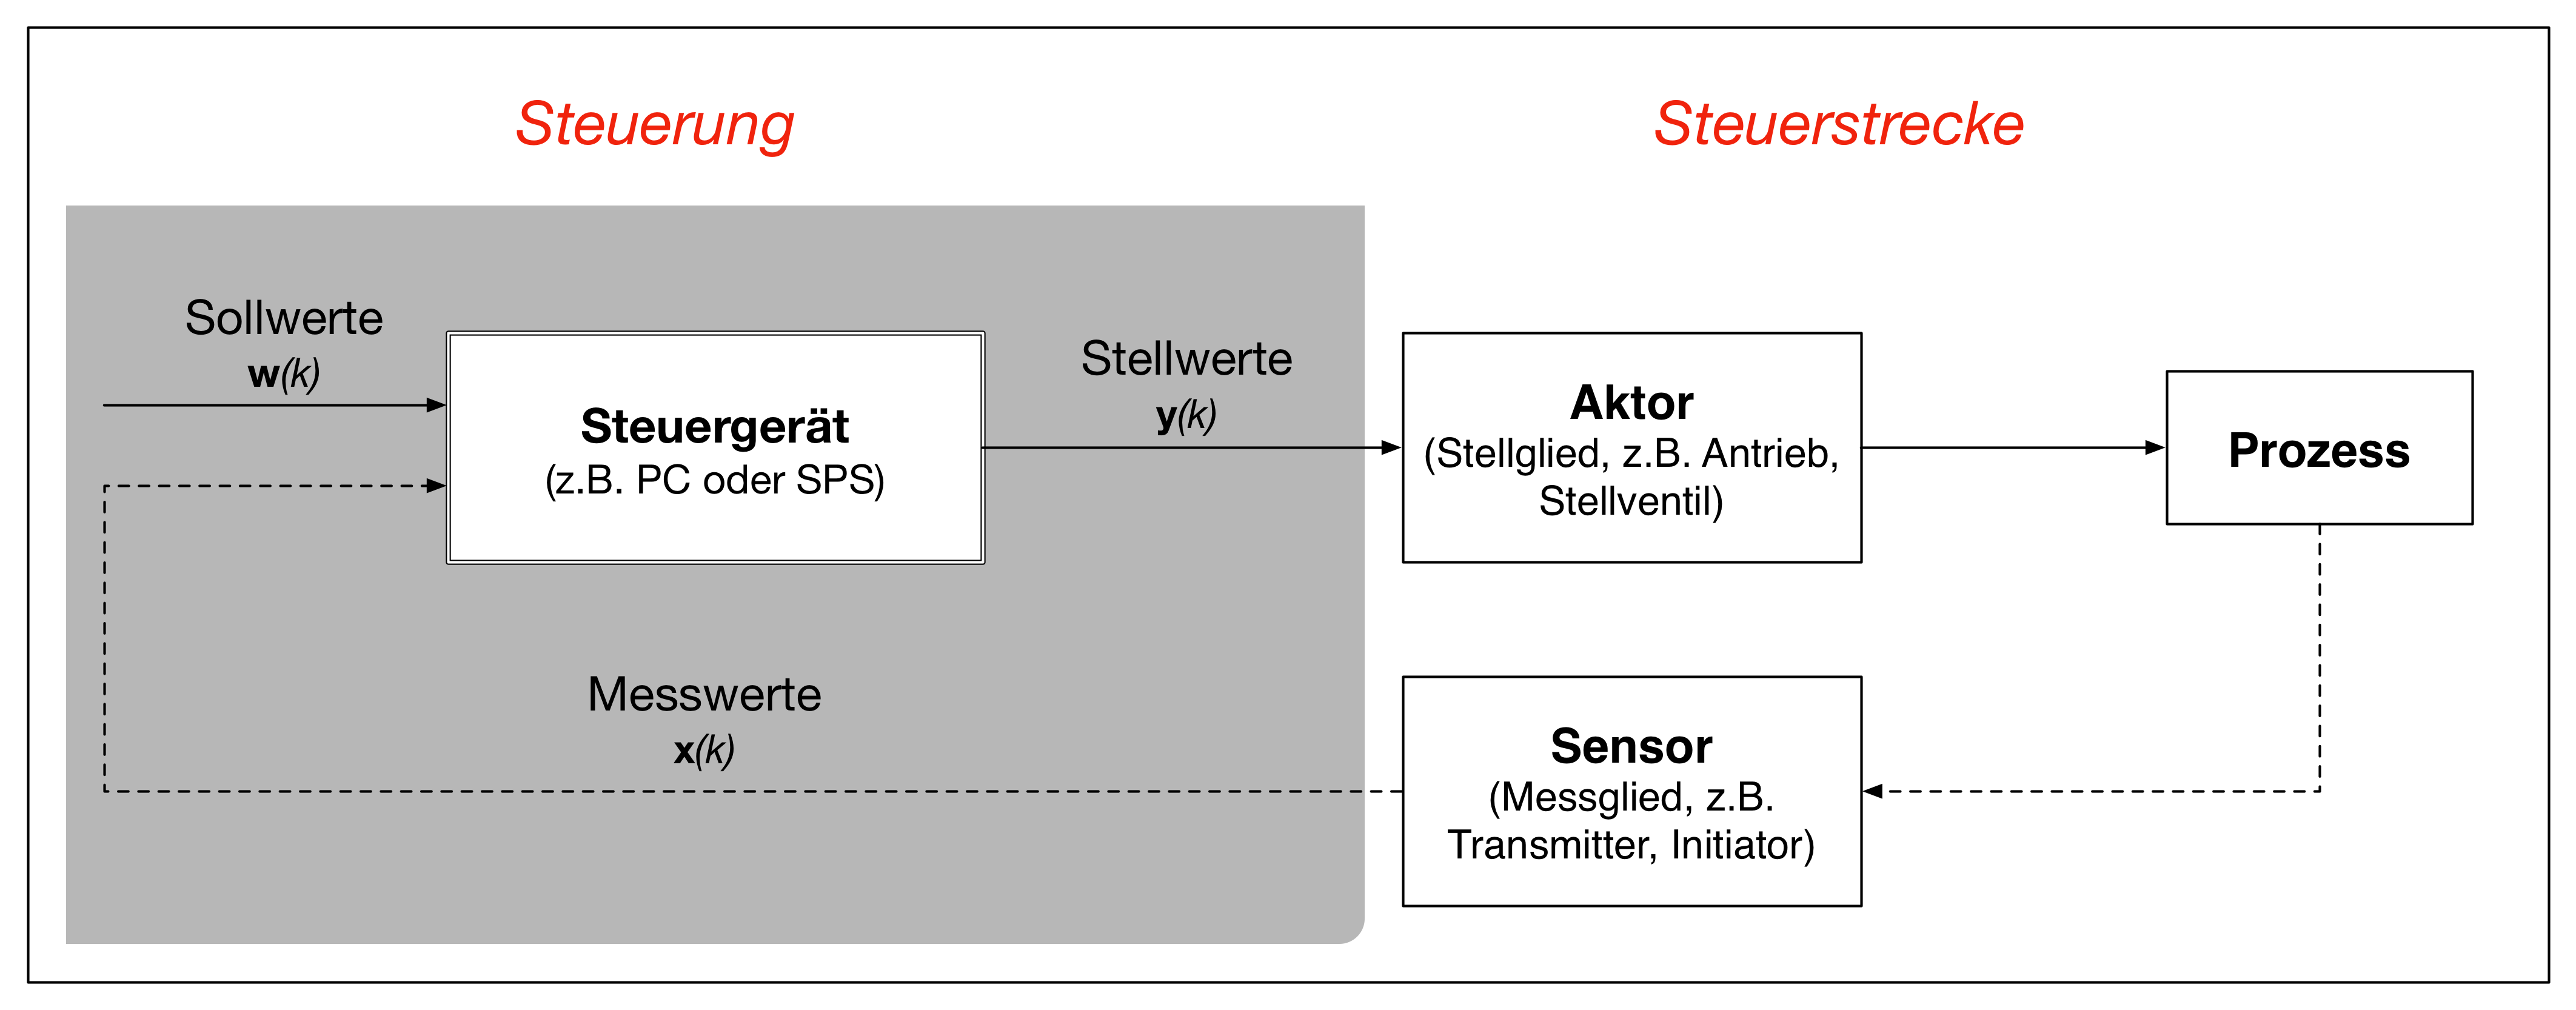
\includegraphics[width=1\textwidth]{graphics/stateoftheart/Aufbau_Steuerkreis_Selfmade.png}
  		\caption{Allgemeiner Aufbau eines Steuerkreises \cite{mseitz_sps}}
			\label{fig:Aufbau_Steuerkreis_Selfmade}
	\end{figure}	
 
 
 Im Detail gehört zum Aufbau einer SPS eine Stromversorgung, eine Verarbeitungseinheit (CPU), digitale sowie analoge I/O Anschlüsse, eine Feldbusschnittstelle und das Programmiergerät, wobei es sich dabei heutzutage eigentlich ausschließlich um einen externen Computer handelt. Die Stromversorgung PS (\textbf{P}ower \textbf{S}upply) wandelt gleichzeitig die Netzspannung in eine 24-V-Gleichspannung um, mit der die Elektronik der SPS versorgt wird.\\
	
	Man unterscheidet drei verschiedene Aufbauarten bei SPSen
	
	\begin{itemize}
  		\item Hardware - SPS
  		\item Slot - SPS
  		\item Soft - SPS
	\end{itemize}

	\textbf{Hardware - SPS}\\\\
	Der im vorigen Abschnitt beschriebene Aufbau einer SPS bezieht sich auf die klassische Aufbauform einer \textit{Hardware - SPS}. Ihre Komponenten sind als gewöhnliche Einsteckkarten in einem Gehäuse oder Schaltschrank angeordnet und sind über einen Rückwandbus miteinander verbunden. Die Hardware - SPS benötigt einen externen PC als Programmiergerät.\\
	
	\textbf{Slot - SPS}\\\\
	Eine Slot - SPS ist eine Einsteckkarte für den PC, welche alle Module einer SPS enthält. Anstatt einer CPU befindet sich ein Co-Prozessor in ihr, auf dem ein eigenes multitaskingfähiges Betriebssystem läuft. Zusätzlich verfügt sie über einen sogenannten multi-ported RAM (ein geteilter Speicher, der sowohl für SPS, als auch für PC zugreifbar ist).\\
	
	\textbf{Soft - SPS}\\\\
	Zu guter Letzt gibt es die Soft - SPS, welche im Gegensatz zu den anderen Steuerungseinheiten eine reine Softwarelösung ist, die komplett auf der CPU des Host-PCs läuft und auch deren Hardware nutzt. Zur Ankopplung der Sensoren und Aktoren ist eine Einsteckkarte zur Feldbuskopplung notwendig, die mit einem Prozessor zur Buskommunikation und einem dual-ported Ram ausgestattet ist.\\
	
	Die Vorteile der SPS im PC ergeben sich hauptsächlich dadurch, dass die rasante Entwicklung der PC-Leistungen für SPSen genau dafür genutzt werden kann.\\
	
	Die Informationsverarbeitung in einer SPS verläuft zyklisch. Die Verarbeitungsschritte lassen sich vereinfacht mit dem EVA - Prinzip beschreiben.
	
	\begin{itemize}
		\item \textbf{E}inlesen der Sensordaten
		\item \textbf{V}erarbeiten der Informationen im SPS-Programm
		\item \textbf{A}usgeben der Soll-Werte an die Aktoren
	\end{itemize}
	
	Die CPU fragt anfangs nacheinander alle Eingangskanäle ab und legt anschließend die Daten in den Arbeitsspeicher - es entsteht das sogenannte \glqq Eingangsabbild\grqq. Hierbei handelt es sich jedoch nicht um die aktuellen, sondern um die zum Abtastzeitpunkt ausgelesenen Werte. Die erstellten Programme werden ausschließlich von der CPU jeweils Schritt für Schritt abgearbeitet. Erst nach Abarbeitung \textbf{aller} Programme werden die im Ausgangsabbild abgelegten Sollwerte nacheinander an die Ausgangskanäle übertragen. \cite{mseitz_sps} \\ 
	
	Kleinere SPS - Hersteller versuchen ihre eigene spezifische Hardware möglichst kompatibel für fremde Software zu produzieren, um mit ihrem Produkt eine möglichst große Zielgruppe anzusprechen. Große Hersteller hingegen möchten ihr System eher geschlossen für den Zugriff mittels fremder Software halten, um die Kundenbindung auf den verschiedensten Ebenen der Automatisierungspyramide zu erhöhen.
	
	\begin{figure}[h!]
  		\centering
    	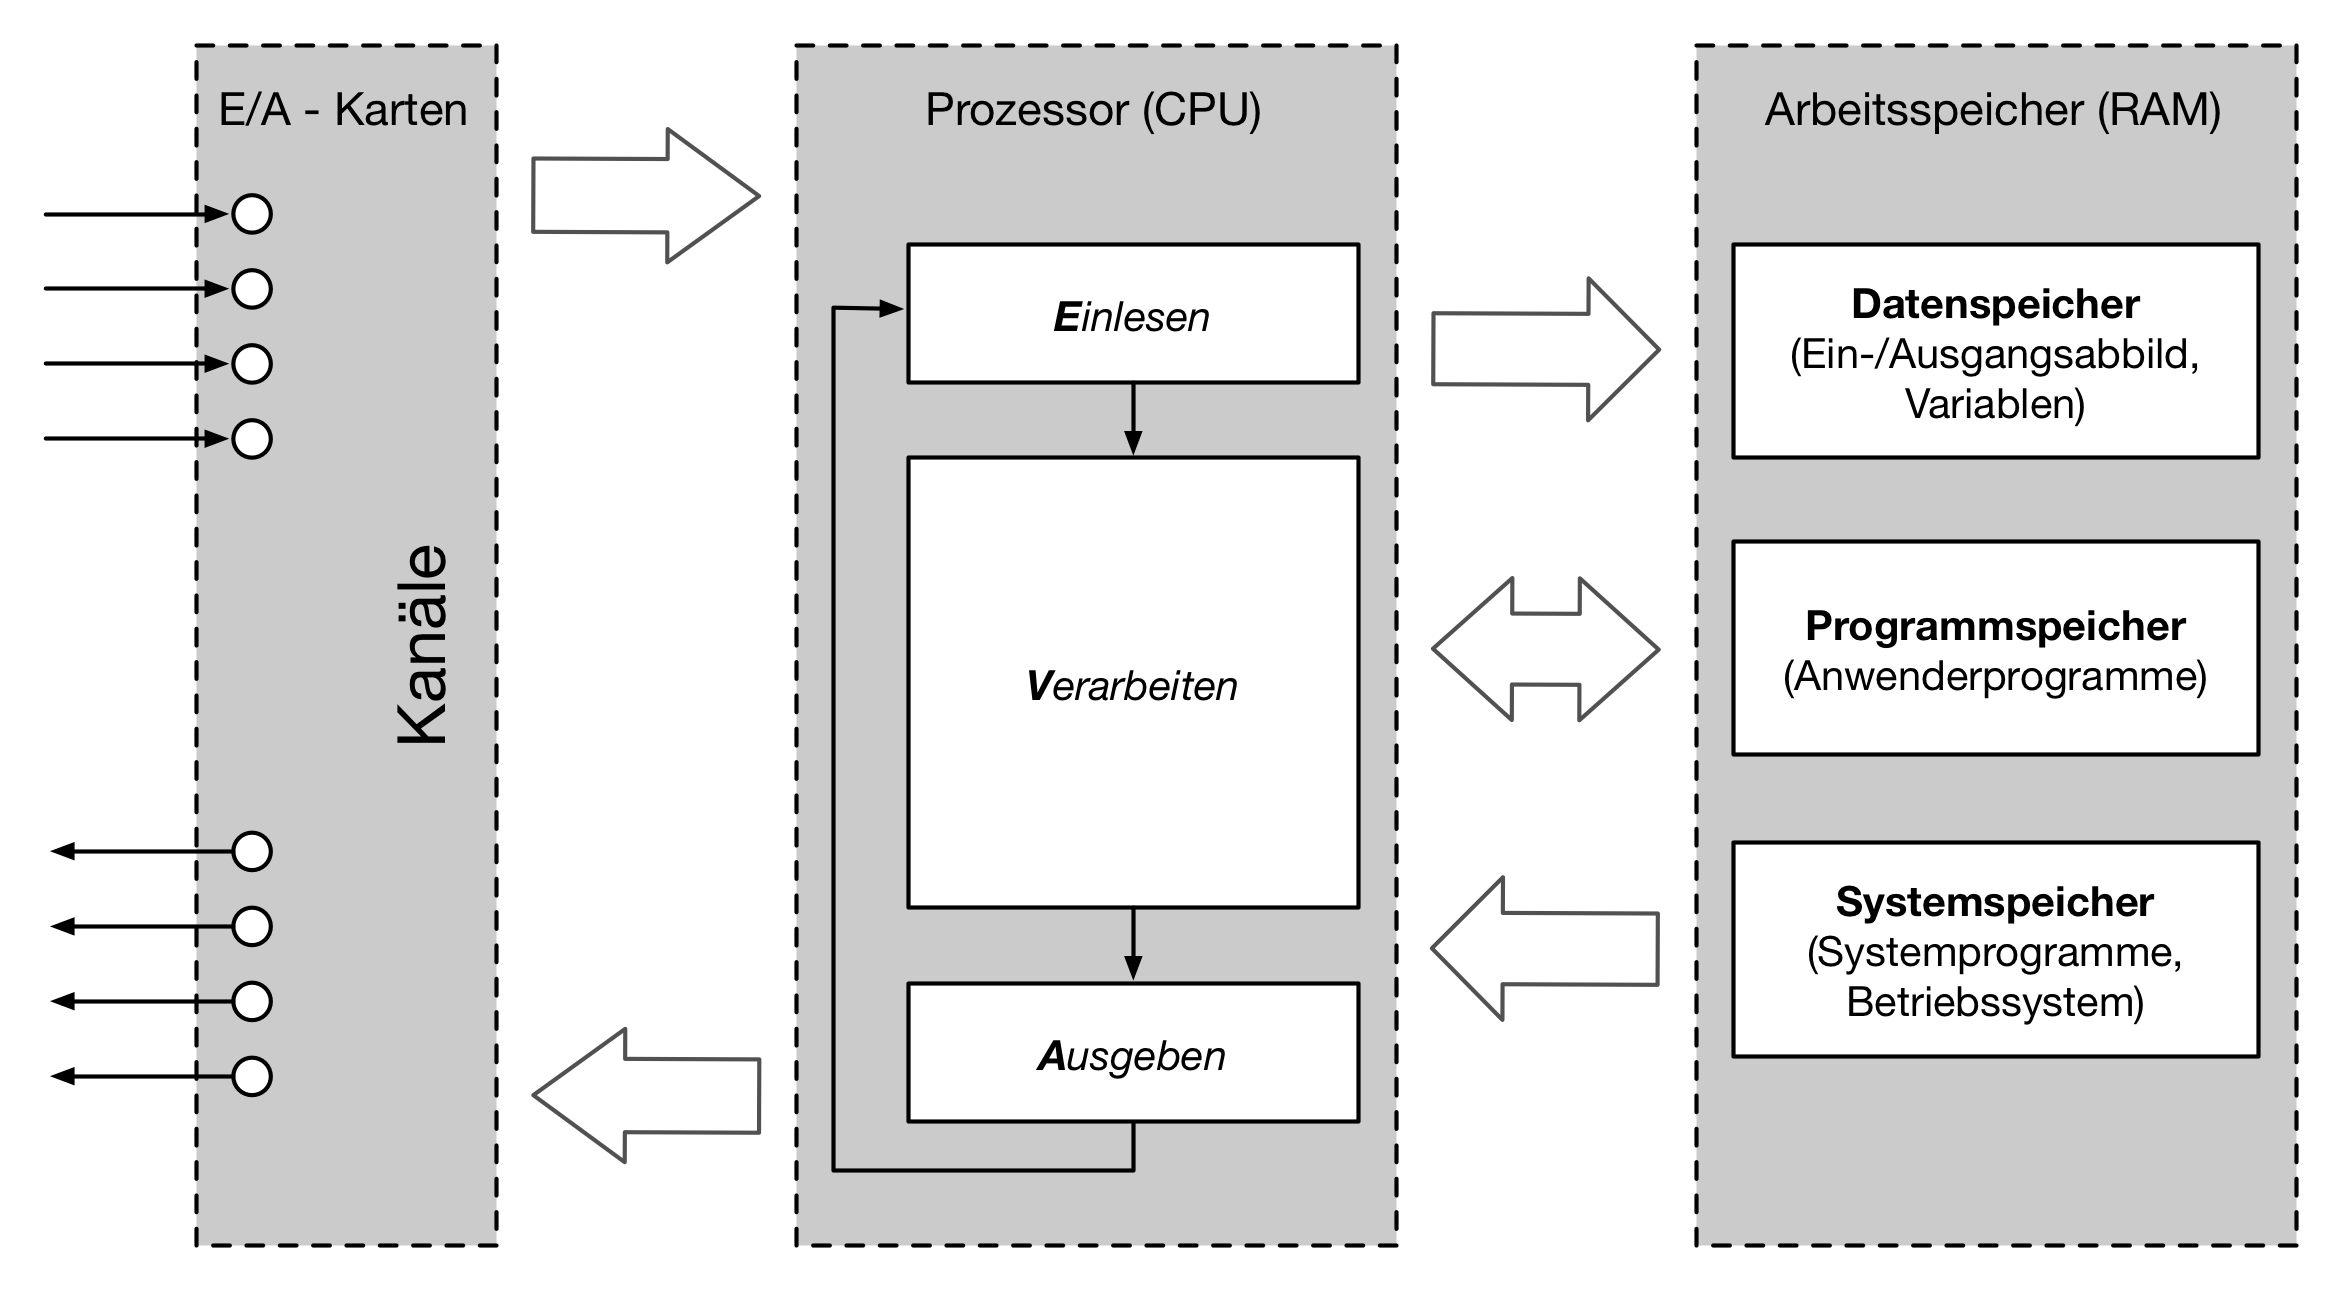
\includegraphics[width=1\textwidth]{graphics/stateoftheart/Signalverarbeitung_Selfmade.png}
  		\caption{Signalverarbeitung und Arbeitsweise einer SPS \cite{mseitz_sps}}
	\end{figure}
		
	% ##############################################################
	% Programmierung einer SPS - Wie funktioniert das grundsätzlich?
	% ##############################################################
	\section{Programmierung einer SPS}

	In der Automatisierungs- und Regelungstechnik gibt es zum Erfüllen der gegebenen Anforderung mehrere Wege um diese zu lösen. Genauer gesagt handelt es sich hierbei um ganze sechs verschiedene Programmiersprachen, um auf jede möglich auftretende sowie spezifische Anforderung individuell eingehen zu können. Diese unterteilen sich wiederum in zwei differenzierbare Untergruppen. So gibt es zum einen die textbasierten Programmiersprachen
	
	\begin{itemize}
		\item[a)] Anweisungsliste (engl. \textit{Instruction List})
		\item[b)] Strukturierter Text (engl. \textit{Structured Text})
		\item[c)] Ablaufsprache (engl. \textit{Sequential Function Chart})
	\end{itemize}

	Im Gegensatz dazu gibt es noch die grafikbasierten Programmiersprachen
	
	\begin{itemize}
		\item[d)] Kontaktplan (engl. \textit{Ladder Diagram})
		\item[e)] Ablaufsprache (engl. \textit{Sequential Function Chart})
		\item[f)] Funktionsbausteinsprache (engl. \textit{Function Block Diagram})
	\end{itemize}
	
	Ziel dieser Vielfalt ist es, eine Vereinheitlichung der Programmierung von SPSen zu erreichen. Der Standard 61131 ist seit 1993 eingeführt und industriell etabliert. Mittlerweile schon in der dritten Edition verfügbar, und somit auch Objektorientierung unterstützend, sind die Programmiersprachen für zentrale und eng gekoppelte Systeme ausgelegt.\\
	
	\textbf{a) Anweisungsliste}\\
	
	Diese textbasierte Programmiersprache nach der Norm IEC DIN EN 61131-3 ist sehr maschinennahe. Vergleicht man die Anweisungsliste aus Abbildung~\ref{fig:Anweisungsliste} mit höheren Programmiersprachen der Informatik, so ist es eine Art Assemblersprache, die normalerweise 1:1 den jeweiligen Maschinencode übersetzt. Es werden die einzelnen Anweisungen in der Reihenfolge geschrieben, wie sie die Maschine (CPU) abarbeiten soll (auch \glqq Stackorientierte Abarbeitung\grqq \space genannt). Ein großer Vorteil gegenüber allen graphischen Programmiersprachen ist die Tatsache, das AWL funktionell über diese hinausgeht, weil beispielsweise ein komplexer Zählvorgang mittels eines Kontaktplans nicht realisierbar sein könnte.	\cite{spslehrgang_struktur, egroetsch_sps}\\

	\begin{figure}[h!]
		\begin{framed}
			VAR\\
			s1: BOOL; \color{gray}//[input] Sensor Deklaration\\ \color{black}
			s2: BOOL; \color{gray}//[input] Sensor Deklaration\\ \color{black}
			s3: BOOL; \color{gray}//[input] Sensor Deklaration\\ \color{black}
			M: BOOL := 0; \color{gray}//[output] Motor Deklaration (muss initialisiert werden)\\ \color{black}
			END\_VAR\\\\
			LD s1; \color{gray}//[load] Lade den boolean-Wert ins Register\\ \color{black}
			OR s2; \color{gray}//Oder-Verknüpfung mit s1\\ \color{black}
			ANDN s3; \color{gray}//Und-Verknüpfung mit invertiertem Eingang\\ \color{black}
			ST \color{gray}//[store] Ergebnis wird in die Variable Motor geschrieben\\
		\end{framed}
		\caption{Beispiel einer Anweisungsliste}
		\label{fig:Anweisungsliste}
	\end{figure}
	
	\color{black}
	\textbf{b) Strukturierter Text}\\
	
	Diese in Abbildung~\ref{fig:StructuredText} angeführte Programmiersprache der Automatisierungstechnik orientiert sich an der Sprache Pascal, enthält aber neben dieser Sprache zugehörigen spezifischen Elementen aber auch noch SPS-typische Elemente. Geeignet ist ST am vorteilhaftesten für Aufgaben mit mathematischem Hintergrund sowie zum Beschreiben komplexer Algorithmen. Auch für Rezept- und Datenverwaltung hebt sich diese Art der Programmierung durch enorme Vereinfachung vor. Typische Anweisungen für ST sind solche, die in höheren Sprachen durch Bedingungen oder Schleifen ausgeführt werden können \cite{grundlagen_automatisierungstechnik}
	\todo[inline]{Schauen ob die Figur \glqq Strukturierter Text\grqq \space an der richtigen Position ist.}
	
	\begin{figure}[h]
		\begin{framed}
		\color{black}
		VAR\\
		s1: BOOL; \color{gray}//[input] Sensor Deklaration\\ \color{black}
		s2: BOOL; \color{gray}//[input] Sensor Deklaration\\ \color{black}
		s3: BOOL; \color{gray}//[input] Sensor Deklaration\\ \color{black}
		M: BOOL := 0; \color{gray}//[output] Motor Deklaration ( muss initialisiert werden)\\ \color{black}
		END\_VAR\\
		M := (s1 OR s2) AND ( NOT (s3)); \color{gray}//ODER-Verknüpfung von s1 und s2, anschließendes UND-Verknüpfung von Ergebnis mit negiertem s3.\
		\end{framed}
		\caption{Beispiel eines strukturierten Textes}
		\label{fig:StructuredText}
	\end{figure}
	
	\color{black}
	\textbf{c, e) Ablaufsprache}\\
	
	Eine Sonderstellung unter den Sprachen zur Programmierung einer SPS nimmt die Ablaufsprache ein.
	\todo[inline]{Ablaufsprache noch genauer beschreiben!}
	\textbf{d) Kontaktplan}\\
	Die Darstellungsart des Kontaktplans ermöglicht SPS-Programmierern ein Programm auf graphischer Ebene zu erstellen und darzustellen. Ein KOP ist einem Stromlaufplan sehr ähnlich, um Programmieranfängern, die beispielsweise nur in der Elektronik tätig sind/waren und noch nie zuvor analytisch hinterfragten Code entwickelt haben, den Einstieg zu erleichtern. Es werden Elemente wie Spulen, Öffner/Schließer, Eingänge/Ausgänge, usw... verwendet, die zu logischen Blöcken zusammengefasst werden können und so einen Teil des gesamten Programms ergeben. Ein Nachteil dieser standardisierten Programmiersprache ist jedoch, dass es nicht für alle möglichen Operationen auch ein einheitliches Symbol in einem Stromlaufplan gibt. Das wiederum bedeutet, dass bei komplexen Steuerungen oft eine Mischung aus KOP und der Funktionsbausteinsprache (FBS) verwendet wird.
	\todo[inline]{Schauen ob das Bild \glqq kop\_Selfmade\grqq \space an der richtigen Position ist.}
	\begin{figure}[h!]
  		\centering
    	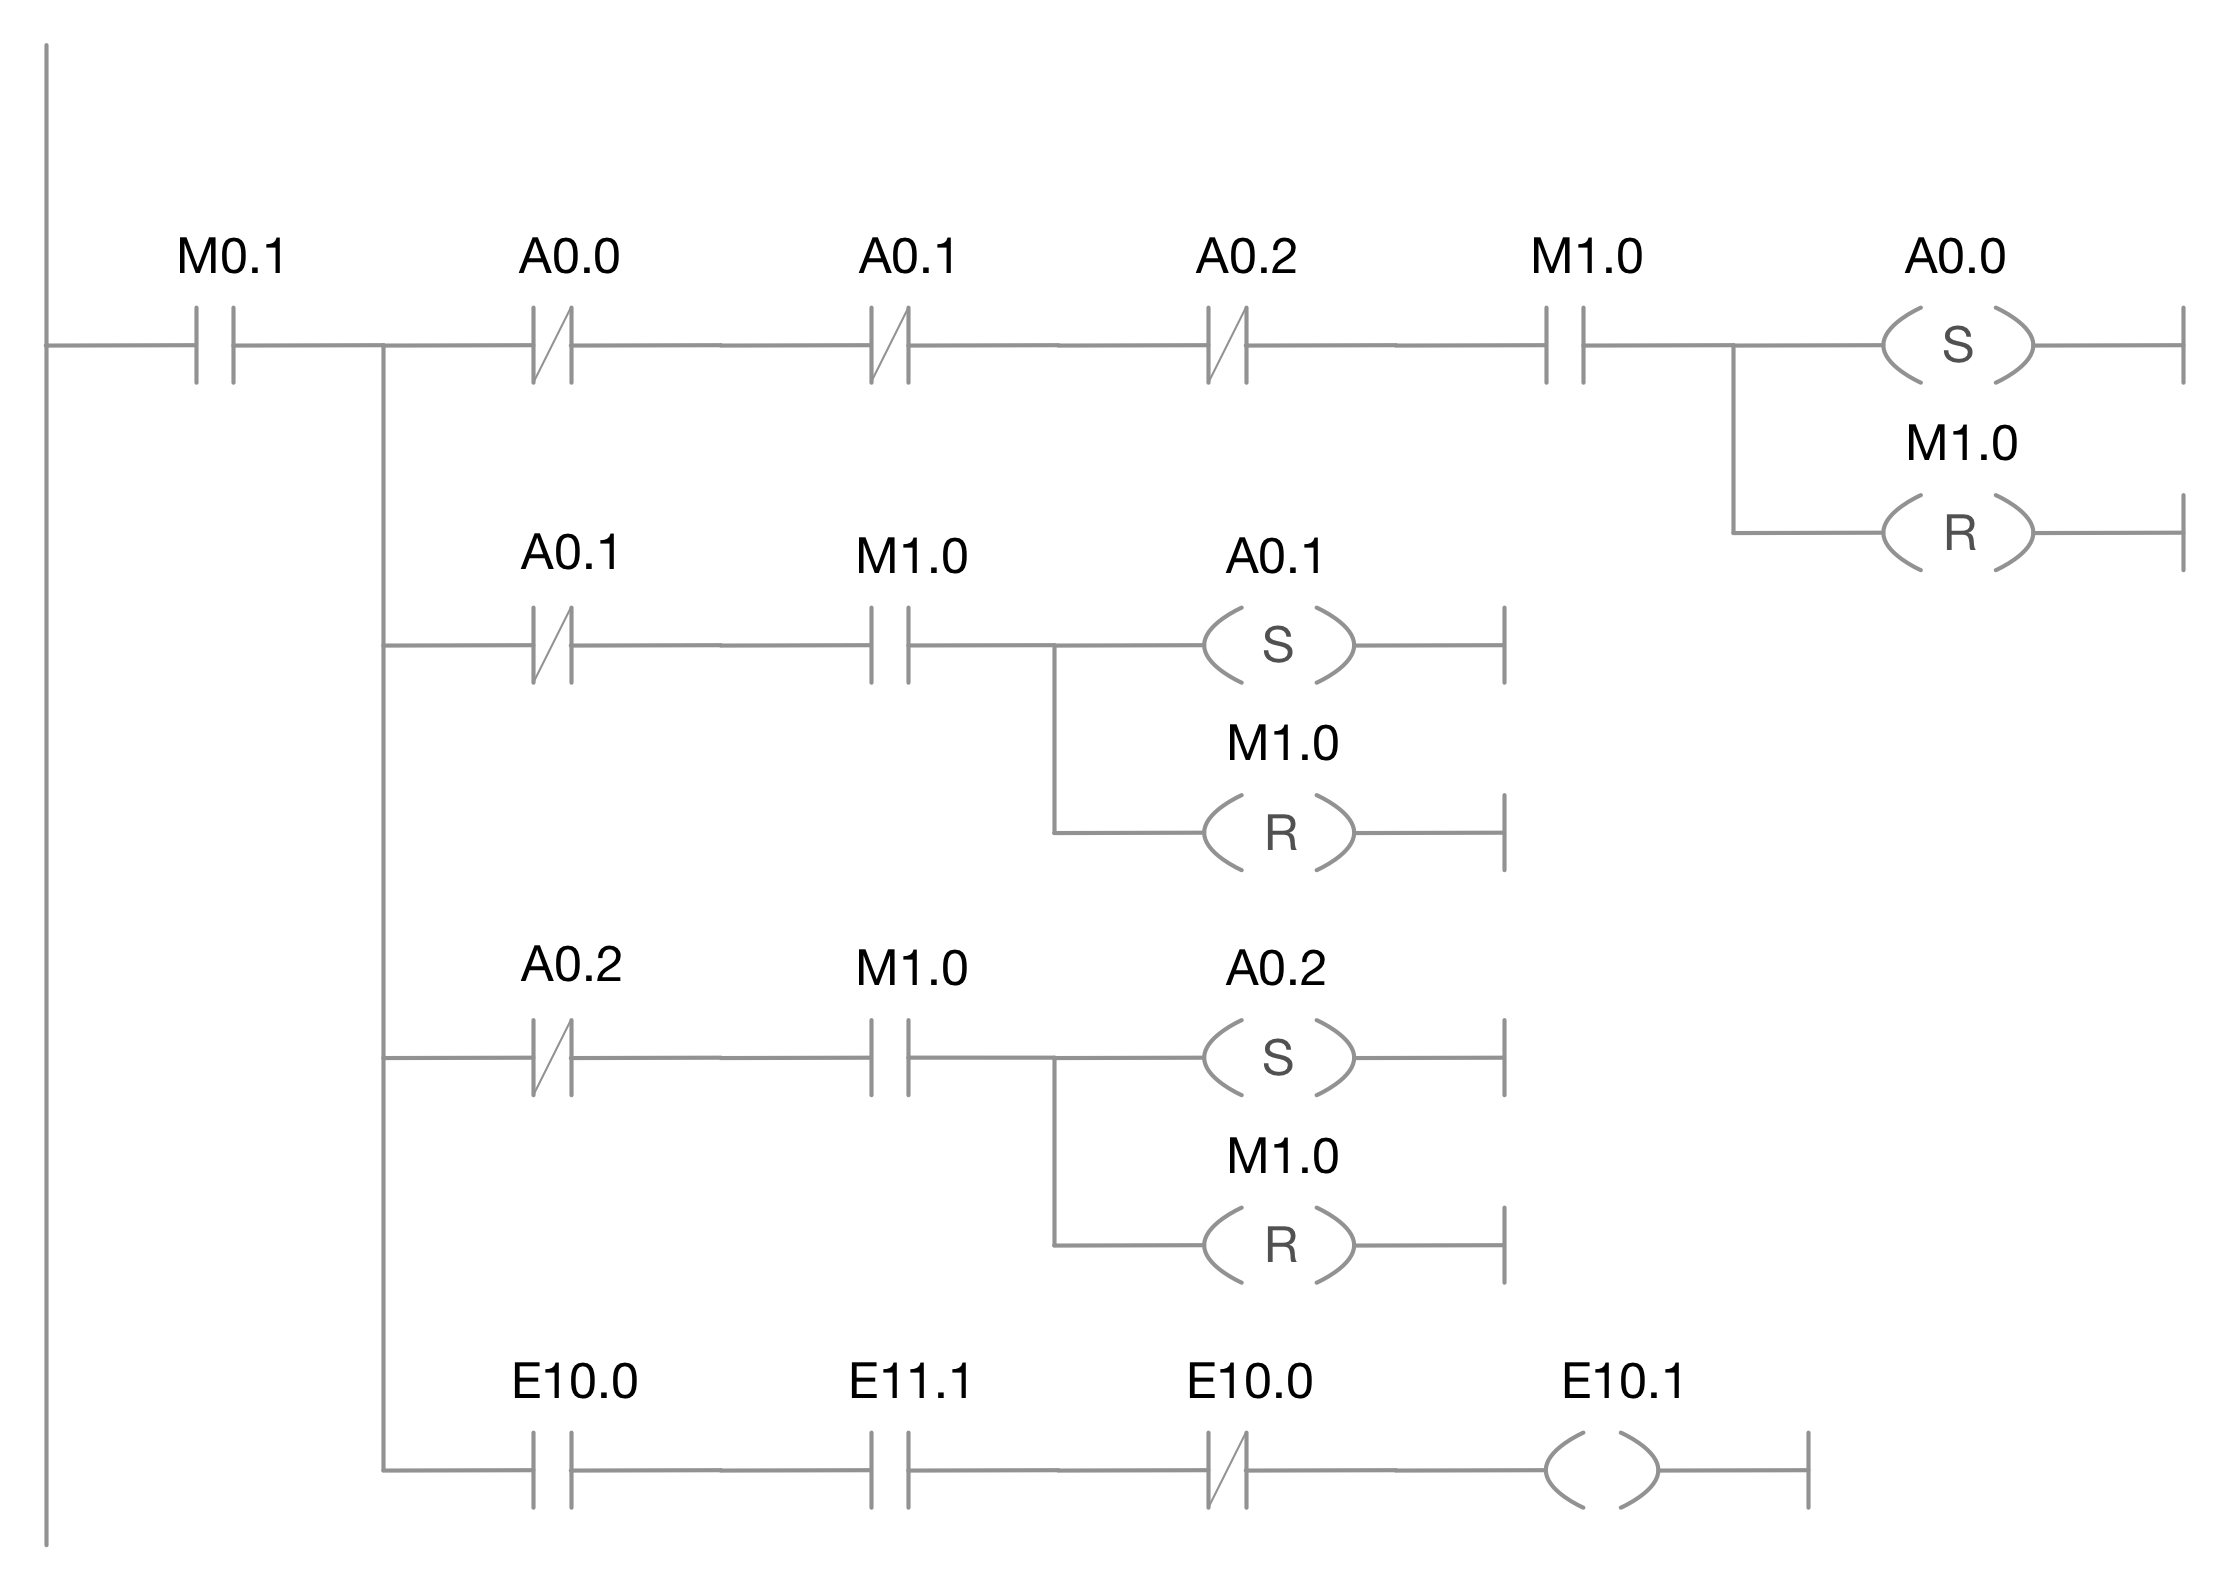
\includegraphics[width=0.8\textwidth]{graphics/stateoftheart/kop_Selfmade.png}
  		\caption{Beispiel eines Kontaktplans \cite{kontaktplan}}
	\end{figure}

	\newpage
	\textbf{f) Funktionsbausteinsprache}\\

	Diese graphische Programmiersprache verwendet für ihre Anweisungen logische Symbole der Boolschen Algebra. Diese Sprache ist insbesondere für Verknüpfungssteuerungen geeignet und deswegen bei Anfängern oder Programmier - Laien beliebt. Durch den einfachen graphischen Aufbau ist die Programmlogik relativ schnell zu erkennen und nachzuvollziehen.

	\begin{figure}[h!]
  		\centering
    	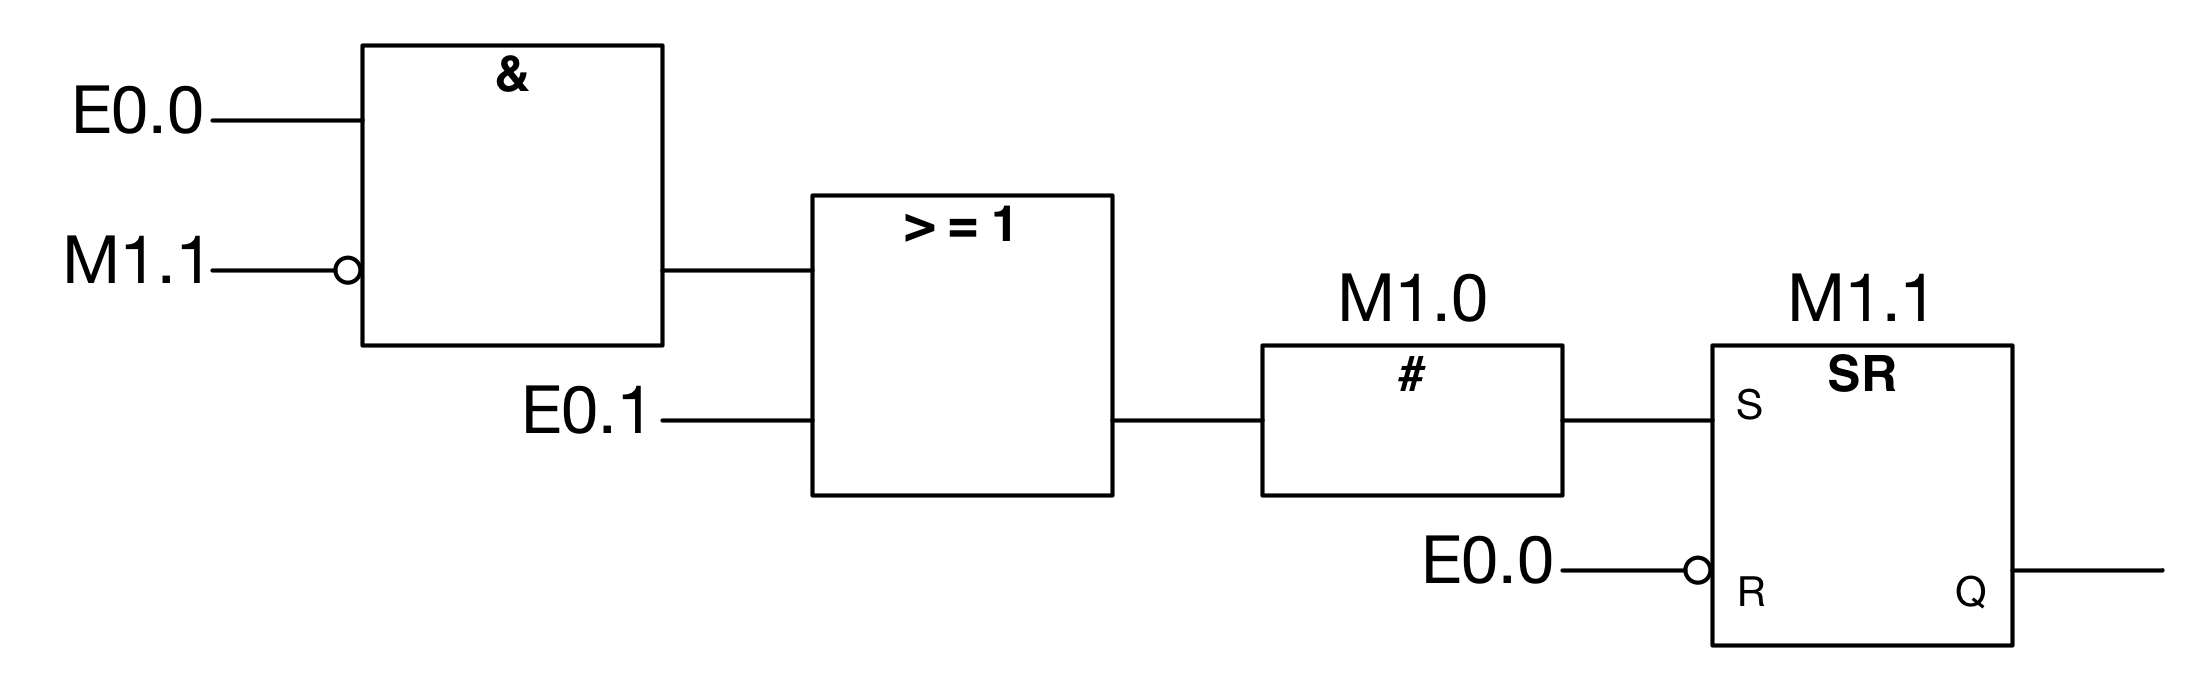
\includegraphics[width=0.8\textwidth]{graphics/stateoftheart/funktionsbausteinplan_Selfmade.png}
  		\caption{Beispiel eines Funktionsbausteinplans \cite{funktionsbausteinplan}}
	\end{figure}

\section{Prozeduren und Rezepte}
\subsection{Prozedur}
Die Prozedursteuerung bestimmt, dass einrichtungsorientierte Aktionen in einer geordneten Folge stattfinden, damit eine prozessorientierte Aufgabe ausgeführt wird. Prozedursteuerungen sind charakteristisch für chargenorientierte Prozesse. Sie sind die Art von Steuerung, die Einrichtungen in die Lage versetzt, einen Chargenprozess auszuführen.\\

%Quelle EN 61522
\begin{figure}[h!]
		\centering
		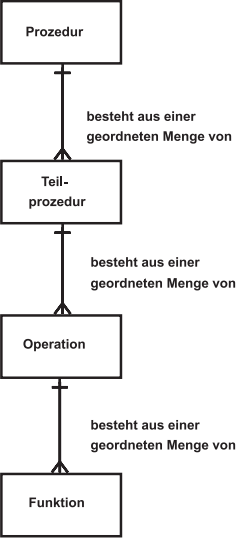
\includegraphics[width=0.4\textwidth]{graphics/stateoftheart/prozedursteuerung.png}
		\caption{Aufbau einer Prozedur}
\end{figure} \todo{Zitat}
\newpage
\textbf{Prozedur}\\
Die Prozedur ist die höchste Stufe in der Hierarchie und legt die Strategie für die Ausführung einer umfassenden Verarbeitungsaktion, wie zum Beispiel der Herstellung einer Charge, fest. Sie wird durch eine geordnete Menge von Teilprozeduren bestimmt. Ein Beispiel für eine Prozedur ist „Produziere PVC“.\\

\textbf{Teilprozedur}\\
Eine Teilprozedur besteht aus einer geordneten Menge von Operationen, die bewirken, dass eine zusammenhängende Produktionssequenz in einer Teilanlage stattfindet. Es wird angenommen, dass zu jeder Zeit immer nur eine Operation in einer Teilanlage aktiv ist. Eine Operation wird in einer einzelnen Teilanlage vollständig ausgeführt. Gleichwohl können mehrere Teilprozeduren einer Prozedur konkurrierend ablaufen, jede in einer anderen Teilanlage.\\ \todo{Zitat}
Beispiele für Teilprozeduren sind:
\begin{itemize}
	\item Polymerisiere Vinylchlorid-Monomer.
	\item Gewinne Vinylchlorid-Rest zurück.
	\item Trockne PVC.
\end{itemize}
\textbf{Operation}\\
Eine Operation ist eine geordnete Menge von Funktionen, die eine größere Verarbeitungssequenz festlegt und die bewirkt, dass die verarbeiteten Stoffe von einem Zustand in einen anderen überführt werden, womit gewöhnlich eine chemische oder physikalische Umwandlung verbunden ist. Häufig ist es erwünscht, die Grenzen einer Operation auf Punkte in der Prozedur zu legen, wo die normale Verarbeitung sicher ausgesetzt werden kann.\\ \todo{ausgesetzt?}
Beispiele für Operationen sind: \todo{Beispiele anhand einer?}
\begin{itemize}
	\item Vorbereitung: Reaktor evakuieren und Reaktorwände mit Antifouling beschichten.
	\item Füllen: Destilliertes Wasser und Lösemittel hinzugeben.
	\item Reaktion: Vinylchlorid-Monomer und Katalysator zugeben, heizen und Absinken des Reaktordrucks abwarten.
\end{itemize}
\textbf{Funktion}\\
Das kleinste Element einer Prozedursteuerung, das eine prozessorientierte Aufgabe ausführen kann, ist eine Funktion. Eine Funktion kann in kleinere Teile unterteilt werden. Die Schritte und Übergänge, wie sie in der IEC 60848 beschrieben sind, dokumentieren eine Methode, um Unterteilungen einer Funktion zu definieren.\\
Ein Schritt kann eine oder mehrere Anweisungen ausgeben oder eine oder mehrere Maßnahmen bewirken, zum Beispiel:\todo{aufzählung..}
\begin{itemize}
	\item Ein- und Ausschalten von Regelungen und zustandsorientierten Arten der Basisautomatisierung und Vorgeben ihrer Sollwerte und ihrer anfänglichen Ausgangswerte.
	\item Setzen, Löschen und Ändern von Alarmgrenzen und anderen Grenzwerten.
	\item Setzen und Ändern von Reglerkonstanten, Betriebsarten von Regelungen und Typen von Algorithmen.
	\item Lesen von Prozessvariablen, wie z. B. Gasdichte, Gastemperatur und Volumendurchfluß von einem Durchflussmesser, und Errechnen des Massendurchflusses durch den Durchflussmesser.
	\item Durchführen der Überprüfung der Bedienberechtigung.
\end{itemize}
Die Ausführung einer Funktion kann resultieren in:
\begin{itemize}
	\item Befehlen an die Basisautomatisierung.
	\item Befehlen an andere Funktionen (entweder in dem gleichen oder einem anderen Einrichtungsobjekt).
	\item der Erfassung von Daten.
\end{itemize}
Das Ziel einer Funktion ist es, eine prozessorientierte Aktion zu bewirken oder zu definieren, wogegen die Logik oder die Folge von Schritten, die die Funktion ausmachen, einrichtungsspezifisch ist.\\
Folgende Beispiele für Funktionen seien genannt:
\begin{itemize}
	\item Vinylchlorid-Monomer zugeben.
	\item Katalysator zugeben.
	\item Heizen.
\end{itemize}

\subsection{Rezept}\todo{Zitat für die Norm}
Rezepte sind Teil der Europäischen Norm EN 61512, welche den Aufbau bei der Chargenorientierten Fahrweise definiert.\\\\
\textit{„Ein Rezept ist eine Gesamtheit, die die Minimalmenge von Informationen enthält, die eindeutig die Herstellungsanforderungen für ein bestimmtes Produkt beschreibt. Rezepte bieten eine Methode, Produkte und die Art, wie diese Produkte hergestellt werden, zu beschreiben“.}\\\\
In der Norm werden die vier Typen von Rezepten, die fünf Kategorien von Informationen, die ein Rezept enthält und wie sich diese Information bei den verschiedenen Rezepttypen verändert, behandelt.\\\\
Es können unternehmensintern noch eigene Rezepttypen verwendet werden, falls die Definierten nicht alle benötigten Anforderungen abdecken, außerdem kann es sein, dass für ein Produkt mehrere Rezepte bestehen, wenn dieses zum Beispiel in verschiedenen Werken produziert wird und dadurch unterschiedliche Abläufe beinhaltet.\\

\subsubsection{Rezepttypen}
%Quelle EN 61522
\begin{figure}[h!]
		\centering
		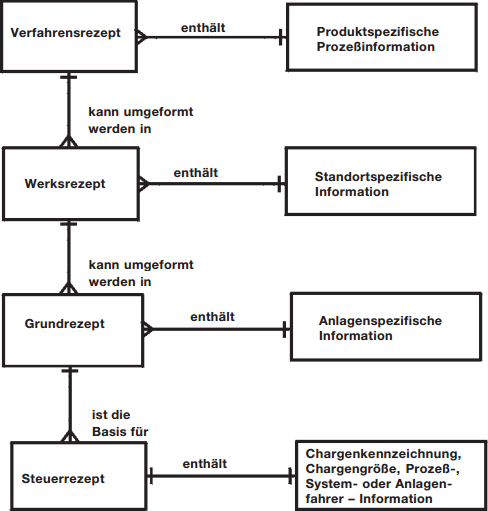
\includegraphics[width=0.6\textwidth]{graphics/stateoftheart/rezepttypen.png}
		\caption{Zusammenhang der Rezepttypen}
\end{figure}
\textit{„Verfahrens- und Werksrezept beschreiben die Vorgehensweise, also wie im Prinzip produziert wird. Grund- und Steuerrezept beschreiben die Aufgabe, also wie mit den tatsächlichen Betriebsmitteln zu produzieren ist.“} \todo{Zitat}
\\\\
\textbf{Verfahrensrezept}\\
Das Verfahrensrezept ist ein Rezept auf Unternehmensebene, das als Grundlage für Rezepte auf niedrigeren Ebenen dient. Das Verfahrensrezept wird ohne spezifische Kenntnis der Anlagenausrüstung erstellt, die zur Herstellung des Produktes benutzt werden wird. Es bestimmt die Rohstoffe, ihre relativen Mengen und die erforderliche Verarbeitung, allerdings ohne Bezug zu einem bestimmten Werk oder der in diesem Werk verfügbaren Ausrüstung. Es wird von Personen mit Kenntnissen der Chemie und den Verarbeitungsanforderungen erstellt, die für das betreffende Produkt typisch sind, und gibt deren Interessen und Überlegungen wieder.\\\\
Das Verfahrensrezept kann für die unternehmensweite Planung und für Investitionsentscheidungen benutzt werden. Es kann ein Teil von Produktionsvorgaben sein oder von solchen in Bezug genommen werden und kann als solches für die Produktionsplanung und zur Information von Kunden und Behörden verwendet werden.
\\\\
\textbf{Werksrezept}\\
Das Werksrezept ist spezifisch für ein bestimmtes Werk. Es ist eine Kombination von werksspezifischer Information und dem Verfahrensrezept. Es wird gewöhnlich aus einem Verfahrensrezept abgeleitet, um die Bedingungen einer bestimmten Produktionsstätte zu erfüllen, und bietet einen für werksbezogene, langfristige Produktionsplanung erforderlichen Detaillierungsgrad.
\\\\
\textbf{Grundrezept}\\
Das Grundrezept ist die Rezeptstufe, die auf eine Anlage oder eine Gruppe von Einrichtungen einer Anlage ausgerichtet ist. Ein Grundrezept kann vom Verfahrensrezept oder vom Werksrezept abgeleitet werden. Es kann mehrere von einem Werksrezept abgeleitete Grundrezepte geben, von denen jedes den Teil des Werksrezeptes abdeckt, der in einer Anlage ausgeführt werden kann. Das Grundrezept kann produktspezifische Informationen enthalten, wie sie zur detaillierten Produktionsplanung erforderlich sind, wie zum Beispiel Informationen über Prozesseinsätze oder Anforderungen an die Einrichtung.\\\\
Das Grundrezept ist eine unverzichtbare Rezeptstufe, da ohne es keine Steuerrezepte erzeugt und daher keine Chargen produziert werden können.
\\\\
\textbf{Steuerrezept}\\
Das Steuerrezept entsteht als eine Kopie einer bestimmten Version des Grundrezeptes und wird anschließend wie erforderlich durch Informationen für Dispositionsplanung und Ausführung verändert, um spezifisch für eine einzelne Charge zu sein. Es enthält produktspezifische Prozessinformationen, wie sie zur Produktion einer bestimmten Charge erforderlich sind. Es bietet den Detaillierungsgrad, wie er zum Start und zur Überwachung der Einrichtungsprozedurobjekte einer Anlage erforderlich ist. Es kann verändert worden sein, um die tatsächlichen RohstoffQualitäten und die tatsächlich eingesetzte Ausrüstung zu berücksichtigen. Die Auswahl von Teilanlagen und entsprechende Skalierung kann jederzeit durchgeführt werden, bevor diese Information benötigt wird.
\subsubsection{Bestandteile des Rezeptes}

\textbf{Rezeptkopf}\\
Die organisatorische Information im Rezept wird als Rezeptkopf bezeichnet. Typische Informationen im Rezeptkopf kann die Rezept- und Produktidentifikation, die Versionsnummer, den Rezeptersteller, das Ausgabedatum, Freigaben, Status und andere organisatorische Angaben enthalten.
\\\\
\textbf{Stoff- und Produktionsdaten}\\
Die Stoff- und Produktionsdaten sind eine Kategorie von Rezeptinformation, die Prozesseinsätze, Prozessparameter und Prozessausstöße umfasst.
Ein Prozesseinsatz besteht aus Bezeichnung und Menge eines Rohstoffs oder eines anderen Betriebsmittels, das zur Herstellung des Produktes erforderlich ist.
Ein Prozessparameter enthält detaillierte Information wie zum Beispiel Temperatur, Druck und Zeit, die wesentlich für das jeweilige Produkt ist.  Prozessparameter können als Sollwerte, Vergleichswerte oder in logischen Bedingungen verwendet werden.
Ein Prozessausstoß besteht aus Bezeichnung und Menge eines Stoffs, die als Ergebnis einer Ausführung des Rezeptes erwartet wird.
\\\\
\textbf{Anforderungen an die Einrichtung}\\
Anforderungen an die Einrichtung schränken die Auswahl der Einrichtungen ein, die schließlich eingesetzt werden, um einen bestimmten Teil der Prozedur durchzuführen. Im Verfahrens- und im Werksrezept werden die Anforderungen an die Einrichtung typischerweise in allgemeiner Weise, wie zum Beispiel zulässigen Werkstoffen und erforderlichen Verarbeitungscharakteristika angegeben.
\\\\
\textbf{Rezeptprozedur}\\
Die Rezeptprozedur beschreibt die Strategie, um einen Prozess durchzuführen. Verfahrensrezeptprozeduren und Werksrezeptprozeduren sind unter Benutzung der im Prozessmodell beschriebenen Ebenen strukturiert, da diese Ebenen es gestatten, den Prozess in einrichtungsunabhängiger Art zu beschreiben. Grundrezeptprozeduren und Steuerrezeptprozeduren werden unter Benutzung der Prozedurelemente des Prozedurmodells beschrieben, da diese Prozedurelemente einrichtungsbezogen sind.

\subsubsection{Einrichtungssteuerung}
Das Steuerrezept selbst enthält nicht genügend Information, um die Anlage zu betreiben. Daher wird es mit der Einrichtungssteuerung, die tatsächlich die Einrichtungen zum Betrieb und zur Produktion von Chargen veranlasst, verknüpft. Die Einrichtungssteuerung wird nicht als Teil des Rezeptes angesehen.
\todo{Quellen haben bei den vorherigen gefehlt}
%Quelle EN 61522
\begin{figure}[h!]
		\centering
		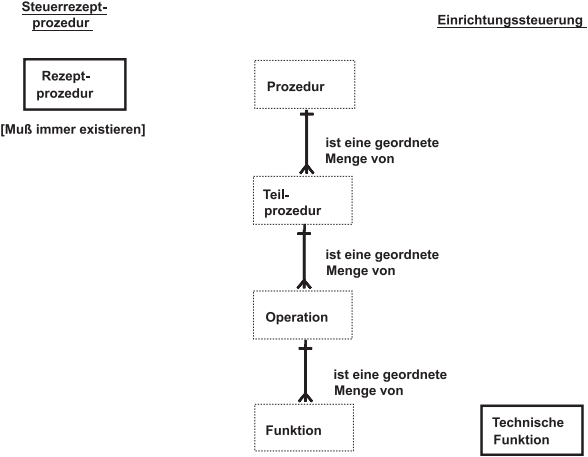
\includegraphics[width=0.8\textwidth]{graphics/stateoftheart/steuerrezeptprozedur_einrichtungssteuerung.png}
		\caption{Abgrenzung von Steuerrezeptprozedur und Einrichtungssteuerung}
\end{figure}


\section{Zenon Wizard}
Ein Zenon Wizard ist ein Programm, das verwendet wird um projektspezifische Daten zu manipulieren, löschen oder erstellen. Dies kann mit oder ohne Benutzeroberfläche geschehen.\\
Der zenon Supervisor enthält schon bei der Installation Wizards zum Importieren sowie auch Exportieren von in XML gespeicherten Daten und zum Erzeugen von Variablen.\\
Der Quellcode der mitgelieferten Wizards kann geöffnet und auch editiert werden. Zenon Wizards können mittels VSTA oder VBA erstellt werden.

\begin{figure}[h!]
		\centering
		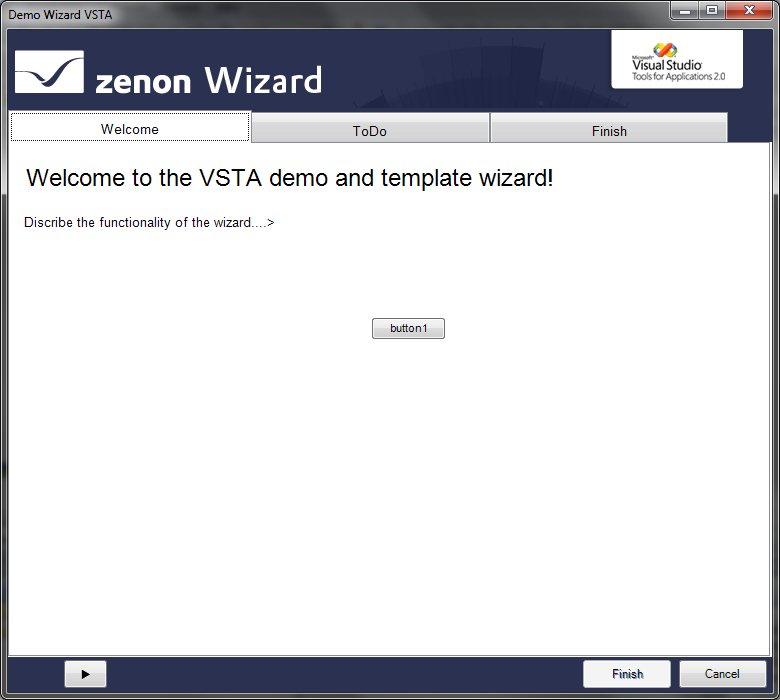
\includegraphics[width=0.8\textwidth]{graphics/stateoftheart/demowizard.png}
		\caption{Beispiel eines VSTA Wizards}
\end{figure}

\subsubsection{VSTA}
VSTA steht für \textit{Visual Studio Tools for Applications}, es ist eine Ansammlung von Werkzeugen zum erstellen von Programmen. VSTA unterstützt die Programmiersprachen Visual Basic .Net und C\#.
VSTA ist in Zenon als Editor integriert.

\begin{figure}[h!]
	\begin{framed}
	\color{black}
		String strName;\\
		zenOn.IDriver Driver;\\
		zenOn.tpKanaltypes ChannelType;\\
		zenOn.IVarType VarType;\\
		zenOn.IVariable Var;\\
		\\
		strName = "Variable";\\
		Driver = proj.Drivers().Item("Treiber");\\
		ChannelType = zenOn.tpKanaltypes.tpSPSMerker;\\
		VarType = proj.VarTypes().Item("Typ");\\
		Var = MyWorkspace.ActiveDocument.Variables().CreateVar(strName, Driver, ChannelType, VarType);
	\end{framed}
	\caption{Anlegen einer Variable in C\#}
\end{figure}

\subsubsection{VBA}
VBA steht für \textit{Visual Basic for Applications} und ist eine Skriptsprache, die hauptsächlich für die Steuerung in Microsoft Office Produkten verwendet wird.
Ein Editor für VBA ist in Zenon integriert.

\begin{figure}[h!]
	\begin{framed}
		\color{black}
		Dim strName As String\\
		Dim Driver As Driver\\
		Dim ChannelType As Integer\\
		Dim VarType As VarType\\
		Dim Var As Variable\\
		\\
		strName = "Variable"\\
		Driver = MyWorkspace.ActiveDocument.Drivers.Item("Treiber")\\
		ChannelType = GetChannelType("SPSMerker")\\
		VarType = MyWorkspace.ActiveDocument.VarTypes.Item("Typ")\\
		Var = MyWorkspace.ActiveDocument.Variables.CreateVar(strName, Driver, ChannelType, VarType)
	\end{framed}
	\caption{Anlegen einer Variable in VBA}
\end{figure}


\section{Visualisierung von Produktionsanlagen}
\subsection{SCADA}
Ein SCADA System, Supervisory Control And Data Acquisition, ist im Allgemeinen eine Sammelstelle für alle aus der Anlagen generierten Werte. Diese Daten müssen dann weiterverarbeitet werden um daraus Analysen zu erstellen.\\
Zu den Elemente eines SCADA Systems gehören:\\
Ein SCADA System besteht aus den folgenden 3 Teilen:
\\
%todo Quelle Scada
%http://www.engineersgarage.com/articles/scada-systems?page=1
%10 März 2015
\textbf{SCADA Master Station Computer Systems}\\
Sammelstelle für Echtzeitdaten, die von RTUs generiert werden. Meist herkömmliche Computer Hardware.\\ \todo{kein Satz}
\\
\textbf{Remote Terminal Units (RTUs)}\\
Sensoren, die physikalische Änderungen in der Anlage mit einem Signalumformer in elektrische Werte umwandelt. Je nachdem was gemessen werden soll, entstehen analoge (Füllstand, Helligkeit, Druck, ...) oder digitale (z.B. Status eines Geräts) Werte.
\\
\textbf{Human-Machine Interface}\\
Aus den gesammelten Daten Analysen (Prognosen, Diagnosen) so aufbereiten, dass sie für den Anwender leicht verständlich dargestellt werden.\\ \todo{umformen}

\subsection{HMI}
Die Visualisierung einer Produktionsanlage ist ein wesentlicher Punkt der Datenverarbeitung und wird oft als Benachrichtigungszentrale benutzt. Meist werden in dieser in Echzeit aktualisierte Statuswerte sowie Benachrichtigungen zu unerwarteten Ereignissen angezeigt. Die hierfür benötigten Daten müssen von der SPS in die Visualisierungssoftware übermittelt werden. Da dies ein sehr aufwendiger Prozess ist, gibt es SCADA-Systeme die all diese Funktionen vereinen.\\
\\
Für dieses Projekt wurde eine Umsetzung in der SCADA Software zenon verlangt, daher wird im weiteren nur noch über die Visualisierung in zenon's HMI System, dem zenon Supervisor, gesprochen.\\
\\

%Quelle http://www.protec.at/dienstleistungen/visualisierung
%Quelle http://www.protec.at/tl_files/protec/uploads/Bilder_Logos/Visualisierung/visualisierung2.jpg
\begin{figure}[hbt!]
 \centering
	\caption{Beispiel Visualisierung in Zenon Supervisor}
\end{figure}


\newpage

\section{Modellbasierte Entwicklung der Steuerung} \label{modellbasierte_entwicklung}
Das Gebiet der modellbasierten Entwicklung bzw. der automatisierten Codegenerierung aus einem Modell als ganzes kann man nicht wirklich als State of the Art erklären.\\
Wenn man sich jedoch die Gebiete als einzelnes anschaut, erkennt man, dass diese im heutigem Betrieb eingesetzt werden. \todo{kann man nicht so schreiben}
\subsection{Modell}
Ein Modell der gesamten Anlage wird schon im frühen Stadium der Entwicklung in Form eines RI-Fließschemas hergestellt, um klar zu definieren, welche Bauteile benötigt werden und welches mit welchem Bauteil verbunden ist. Dies ist nur das erste Modell das in der Industrie eingesetzt wird.\\
\\
Oft werden aber mehr Informationen benötigt als im RI-Fließschema ersichtlich sind, weswegen man auf eine andere Methode umsteigen muss ein Modell abzubilden.\\
Auf die gängigsten Methoden (XML, Ontologie, UML) wird in den nächsten Punkten genauer eingegangen.
\subsection{XML}
XML ist ein textbasiertes Dateiformat, dass obwohl es für Dokumente gedacht ist, oft für das Abbilden von Daten Strukturen verwendet wird.
\\
Ähnlich wie in HTML verwendet auch XML Tags, der Unterschied besteht darin, dass XML keine vorgefertigten Tags besitzt und der Benutzer diese erstellt. Genau diese Benutzerdefinierten Tags ergeben die XML Struktur, welche, was essentiell ist, von alleine nur ein Textfile ist und keine Funktionen besitzt. \todo{Satz kann nicht so bleiblen}
\newpage
\lstinputlisting[language=XML,belowcaptionskip=5pt,frame=bt,caption=XML Sample Code]{extra/sample.xml}
Der Aufbau einer XML Datei ist leicht zu erklären: Es gibt 1 rootElement, dass den Anfang und das Ende des Inhaltes markiert. Zwischen dem Start- und Endtag befinden sich weitere Tags, die das Dokument oder die Struktur genauer beschreiben. Jeder Tag kann Attribute besitzen die es weiter definieren. Zwischen einem Start- und Endtag können sich entweder weitere Tags oder einfacher Text befinden.
\\
Einsatz findet XML meist in Programmen oder Webseiten, die größere Mengen an Daten bzw. Befehle Systemunabhängig übertragen sollen. Grund dafür ist unter anderem die Tatsache, dass Mensch und Maschine die Datei ohne Übersetzung bzw. Kompilieren lesen und verstehen kann.\\
Doch auch wenn ein Mensch XML-Dateien lesen kann, dauert es länger die Struktur eines Textes, im Vergleich zu einer grafischen Darstellung, zu verstehen.\\  \todo{Mensch?}
Dafür gibt es andere Werkzeuge, die auf XML basieren, aber eine grafische Darstellung erzeugen.
\subsection{Ontologie}
%todo Quelle Ontologie
%http://plato.stanford.edu/entries/logic-ontology/
Eine Ontologie ist ein auf XML basierendes Konstrukt, dass einem das Abbilden von Dingen und deren Relationen ermöglicht. Um solch komplexe Zustände darzustellen, stehen neben einfachen Entitäten (Dinge) auch Eigenschaften zur Verfügung.

\begin{displayquote}... we have at least two parts to the overall philosophical project of ontology: first, say what there is, what exists, what the stuff is reality is made out off, secondly, say what the most general features and relations of these things are.
\end{displayquot}

\textbf{Allgemeiner Aufbau einer Ontologie}\\
Das Modell an sich ohne zusätzliche Attribute oder Eigenschaften ist vom Aufbau her so zu erklären: Es gibt ein 'Thing', von dem alles aus geht \todo{keine Klammer} (das root Element bei XML). Von diesem Punkt aus können weitere Entitäten abgeleitet werden \todo{keine Klammer} (Eine Vererbung, vergleichbar mit einem Stammbaum). Die neu erstellte Entität ist immer noch ein Thing, jedoch genauer definiert. Es gibt keine Grenzen oder Vorschriften, in welche Tiefe diese Definition gehen muss. Daher kann dies für sehr komplexe aber auch simple Modelle eingesetzt werden.\\

\begin{figure}[hbt!]
 \centering
  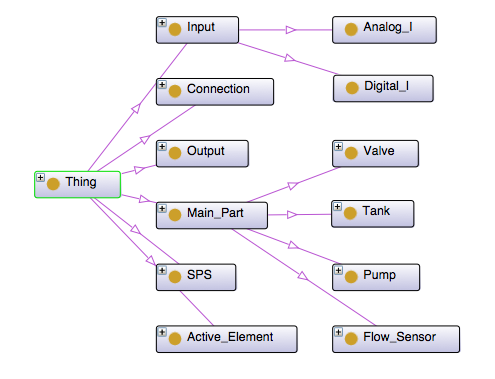
\includegraphics[width=1\textwidth]{graphics/stateoftheart/Ontology_Aufbau}
  \caption{Aufbau einer Ontologie}
	\label{fig:Ontology_Aufbau}
\end{figure}

Wie in Abbildung~\ref{fig:Ontology_Aufbau} zu erkennen erhält man so die Struktur des Modells, jedoch werden oft weitere Informationen zu den einzelnen Objekten/Entitäten benötigt, welche als Eigenschaften abgespeichert werden.\\
Dies ermöglicht ein Modell aufzubauen, dass nicht nur die Struktur abbilden, sondern komplexe Netzwerke konstruieren kann.\\
\\
\noindent \textbf{Objekt Eigenschaften}\\
Objekt Eigenschaften werden benötigt um Relationen zwischen den einzelnen Objekten genauer zu beschreiben.\\
\\
Allgemeine Definition:\\
\textbf{Domain} -> \textbf{Name} -> \textbf{Range}\\
KlasseA -> Eigenschaft -> KlasseB\\
\\
Wie kann man einen Tank mit einer Pumpe verbinden? \todo{Frage geht nicht} Genau dafür gibt es Objekt Eigenschaften. Für diesen Zweck kann man eine Eigenschaft mit dem Namen 'verbunden\_mit' erstellen, und diese dann dem Tank beifügen. So ergibt sich die Relation:\\
Tank -> verbunden\_mit -> Pumpe\\
\\
\textbf{Daten Eigenschaften}\\
Daten Eigenschaften werden benötigt um Objekte genauer zu beschreiben. 
\\
Beispiel für ein Modell einer Produktionsanlage ist es etwaige Sensoren im Modell einen Wertebereich festzulegen in welchem dieser arbeitet bzw. was für Werte dieser sammelt oder zurückgibt: Ein Füllstandsensor mit einem Wertebereich von 4-20V, wobei 4V=Leer und 20V=Voll bedeutet, kann in einer Ontologie mit wenigen Data Properties abgebildet werden.

\subsection{UML}
UML ist, wie eine Ontologie, eine auf XML basierte Modellierungssprache.
%TODO Quelle UML
%Quelle OMG Unified Modeling LanguageTM (OMG UML), Infrastructure
Das Ziel von UML ist es, System Architekten, Software Ingenieuren und Software Entwicklern ein Werkzeug zur Analyse, Design, Implementation von Softwarebasierenden Systemen, sowie für Modell Entwicklung und ähnliche Prozesse zu bieten.\\
\\
Mit Hilfe von UML können viele verschiedene Arten von Diagrammen erstellt werden, für dieses Projekt relevant ist jedoch nur das Klassendiagramm und das Aktivitätsdiagramm, daher wird im weiteren nur auf diese 2 Arten genauer eingegangen.\\
\\
\textbf{Klassendiagramm}\\
\\
Neben einer einfachen Abbildung der Anlage kann man ein Activity Diagram verwenden um beispielsweise einzelne Phasen oder ganze Rezepte abzubilden.\\
\\
\textbf{Aktivität}\\
%TODO Quelle Activity
%Quelle http://timpt.de/topic35.html
Ein Aktivitätsdiagramm beschreibt das Verhalten von Systemen auf Grundlage von vorgegebenen Regeln. 

\begin{figure}[hbt!]
 \centering
  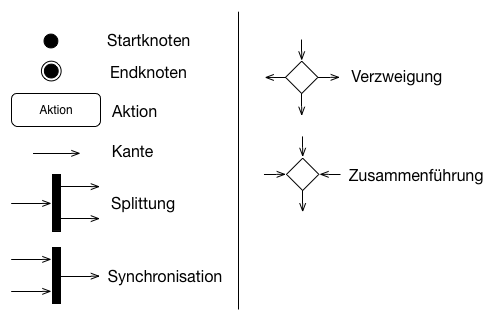
\includegraphics[width=1\textwidth]{graphics/stateoftheart/Activity_Elemente}
  \caption{Basis Elemente eines Aktivitätsdiagramm}
\end{figure}
%Quelle OMG Unified Modeling LanguageTM (OMG UML), Version 2.5
%Als Zitat lassen und das Beispiel auf Deutsch dann erklären (Eng. Begriffe verwenden)
\begin{displayquote}An Activity is a kind of Behavior that is specified as a graph of nodes interconnected by edges. A subset of the nodes are executable nodes that embody lower-level steps in the overall Activity. Object nodes hold data that is input to and output from executable nodes, and moves across object flow edges. Control nodes specify sequencing of executable nodes via control flow edges. Activities are essentially what are commonly called “control and data flow” models. Such models of computation are inherently concurrent, as any sequencing of activity node execution is modeled explicitly by activity edges, and no ordering is mandated for any computation not explicitly sequenced.\\
Activities may describe procedural computation, forming hierarchies of Activities invoking other Activities, or, in an object- oriented model, they may be invoked indirectly as methods bound to Operations that are directly invoked. Activities may be applied to organizational modeling for business process engineering and workflow. In this context, events often originate from inside the system, such as the finishing of a task, but also from outside the system, such as a customer call. Activities can also be used for information system modeling to specify system level processes.\\
\\
Activity Nodes\\
ActivityNodes are used to model the individual steps in the behavior specified by an Activity.\\
\\
Activity Edges\\
An ActivityEdge is a directed connection between two ActivityNodes along which tokens may flow, from the source ActivityNode to the target ActivityNod.\\
\end{displayquote}

%Quelle http://www.uml-diagrams.org/shopping-process-order-uml-activity-diagram-example.html?context=activity-examples
\begin{figure}[hbt!]
 \centering
  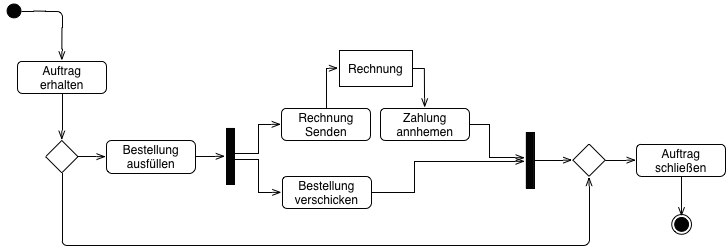
\includegraphics[width=1\textwidth]{graphics/stateoftheart/Activity_bsp}
  \caption{Beispiel für ein Aktivitätsdiagramm}
\end{figure}
%
\subsection{OPC}
%TODO OPC
OLE for Process Control\\
Object Linking and Embedding for Process Control (OPC)\\
XML für Industrie. 
\newpage
\section{Zusammenfassung}

Dieses Kapitel zeigt die Entwicklung und den aktuellen Stand der Technik bezüglich der Anlagen- und Verfahrenstechnik sowie der modellbasierten Entwicklung von Steuerungen für Produktionsanlagen. \\\\
Wie sich herausgestellt hat, ist die Codegenerierung für SPS in Produktionsanlagen heutzutage nicht State Of the Art. Bei Änderungen wie dem Hinzufügen oder Entfernen von Teilen muss ein Großteil des Programm-Codes neu implementiert werden. \\\\
%Um eine Codegenerierung für SPSn in Produktionsanlagen  
%„“
Die Idee ist, diesen Implementierungsschritt auf einer Laboranlage zu automatisieren. Der SPS Code soll auf einem Ontologie-basierten Informationsmodell, um das Konzept von Produktionssystemen zu beschreiben sowie einem Aktivitätsdiagramm, um die Prozeduren zu definieren, generiert werden. Wenn es nun zu Änderungen der Produktionsanlage kommt, können diese im Modell angepasst werden und durch eine Codegenerierung der nötige Implementierungsschritt automatisiert werden. Zusätzlich soll die Integrierbarkeit des Codes in eine Steuerungsapplikation mit Visualisierung mittels der Software zenon von COPA-DATA getestet werden.\\\\
Im Rahmen des Projekts Batch\_it soll eine Laboranlage konzeptioniert und aufgebaut werden. Als weiteres wird eine Steuerungsapplikation mit Visualisierung mithilfe der Software zenon erstellt werden. Dies umfasst das Implementieren von Prozeduren und Rezepten nach dem IEC 61512 Standard. Hierbei handelt es sich um Funktionen wie z.B. das Pumpen von Flüssigkeiten von Tank zu Reaktor. Im letzten Schritt wird die modellbasierte Entwicklung der Steuerung umgesetzt. Dabei wird einen Ontologie erstellt, welche die Laboranlage abbildet und ein Aktivitätsdiagramm, welches die Prozeduren definiert. Anhand dieser wird einen Codegenerierung für die Steuerung der Anlage mittels des zenon Wizards implementiert.\\\\
\textbf{Forschungsfragen}\\\\
%Mit welchen Technologien ist die Implementierung von Code einer SPS einer Chargenprozessanlage automatisierbar? \\\\
Wie genau muss die Chargenprozessanlage abgebildet werden um eine Codegenerierung zu ermöglichen? \\\\
Welche Funktionalität kann durch die modellbasierte Entwicklung der Steuerung abgedeckt werden?\\\\
Wie ausführlich funktioniert die Integrierung der Codegenerierung in die Software zenon von COPA- DATA? 